\section{A theoretical model of poachers, traders, and farmers}

Our framework follows \cite{damania_economics_2007}, with a poaching cost structure adapted to fisheries. The model develops a three-stage dynamic, game theoretic, bioeconomic model. The value chain for poached animal products comprises poachers, middlemen traders, and end markets. As a small number of actors characterizes many wildlife markets, the model features a vertical monopoly and looks at the consequences on wildlife population stocks of the introduction of a farmed substitute. In this setting, farmers compete on end markets with traders in quantity and price. In the original model, price competition unambiguously results in larger harvests than in the vertical monopoly case. Therefore, while quantity competition reduces poaching, the threat of a population collapse in the price-setting case should warrant a cautious approach to conservation farming. We argue that this conclusion is erroneous, as the intricacies of imperfect substitutability and market dynamics have not been properly accounted for in the original model. As a matter of fact, standard economic intuition regarding price-setting competition in the homogeneous goods case does not directly apply here, as fishing costs rise as the stock decreases, limiting the ability of the trader to flood the market. We show that scenarios exist where any type of competition unambiguously leads to positive conservation outcomes, i.e, reduced poaching and larger steady-state stocks. We amend the original results and use this model for simulation. 

First, poachers illegally harvest wildlife resources. Second, they sell their catch to a monopsonistic buyer. Third, the buyer sells catches on a monopolistic market, which is not accessible to poachers. We label this value chain 'vertical monopoly' as a reference case. We then look at the impact of introducing a competitor on the end market, the farming sector. 

%For comparison, we look at the impact of conservation farming on several other market structures. We model an open-access fishery, where the middlemen traders disappear and poachers sell their catch on a perfectly competitive market. As Damania and Bulte (19), we model the case where a middleman trader exists and sells the catch on a perfectly competitive market. 

%\subsection{The open access fishery model}

%First, consider an open-access fishery, where fishermen optimally determine effort to maximize their profits and sell their catch without an intermediary.


\subsection{Entry in the fishery and poaching supply}
We denote the fishing effort by $E$, which is measured in the number of vessel trips. Entry in the poaching sector, $\dot{E}$, is a function of payoff and an adjustment parameter.  Harvest, $q$, follows the Gordon-Schaefer  dynamic biomass model  $q = \sigma x E$, with $\sigma$ the (stock-independent) catchability coefficient, and $E$, effort
%\cite{Clark}
The payoff is determined by the price paid to the poachers $s$ minus the cost of effort. We adopt a disagregated view of the fishery, and consider increasing marginal costs of effort, as individuals have to be attracted from other activities with increasing opportunity costs. To account for energy costs, we derive a modified version of this model using a linear-quadratic cost function (see [37, 53]). Entry happens as long as the profit of the marginal poacher is positive : 
\begin{equation}
    \dot{E}= \eta \frac{d\Pi}{dE} = \eta \frac{d}{dE}\left[ sq-W_1 * E - W_2E^2\right]
\end{equation}
%reach a closed form solution for the optimal $E$ such that it increases in the price paid to poachers and stock.

The resource stock biomass $x$ follows a logistic growth curve and is harvested. Overall, the dynamics are: 
\begin{equation}
    \dot{x} = g(x) - q = rx\left(1 - \frac{x}{K}\right) - \sigma x E
    \label{eq:growth}
\end{equation}
Where $r$ is the intrinsic population growth rate,  and $K$ is the carrying capacity. 

Fishermen enter the fishery as long as the marginal profit from selling to traders along the vertical value chain is positive. As the resource is in open access from the fishermen poachers maximize their instantaneous profit with respect to effort. The optimal effort and aggregate supply of poached fish is:
\begin{align}
    \frac{d \Pi}{d E} = 0
    \Rightarrow & E^* = \max\left( 0, \frac{s \sigma x  -W_1}{2W_2} \right)\\
    \Rightarrow & q^* = \max\left(0, \frac{s\sigma^2 x^2 - W_1\sigma x}{2 W_2}\right)
    \label{eq:poachers_supply}
\end{align}
Given the linear quadratic nature of the costs, there is no effort or catch for low stock levels and/or low prices. Effort and catch increase with the price paid to poachers, $s$.


%The steady state is defined by $\dot{E}=\dot{x}=0$. Plugging the optimal effort in the harvest function yields the supply of the poaching sector and steady state stock in \textbf{open acces}:

%\begin{align}
%   \text{Poaching in} \text{ \textbf{open access} : }
%   q^W =& \sigma  x E = \frac{s \sigma^2 x^2}{2W} \\
%    \label{eq:poachers_supply}
%    \text{Steady state stock} \text{ in \textbf{open access } : }
%    x^*=&\frac{2WrK}{s\sigma^2K + 2Wr}
%\end{align}

%Notice that if prices drop, harvest decreases, and the steady state stock increases.


%\subsection{Wildlife commodity traders as price takers}
%In this part of the model, we introduce a new actor: a wildlife trader buys totoaba from poachers. 

%The trader maximizes profit by determining the price paid to poachers, taking market prices for totoaba as given. Recall that the quantity produced, for the marginal unit of effort to not earn rent is $q^W$. Using $c$ as a transportation and transaction cost : 
%\begin{equation*}
%    \Pi^W= Pq^W - sq^W = (P  -c - s)\frac{s\sigma^2 x^2}{2W}
%\end{equation*}
%We assume the inverse demand function is linear : 
%\begin{equation}
%    P^m = \alpha^m - \beta^m q^W
%\label{eq:inv_demand_monop}
%\end{equation}

%Using $q^W$ and optimizing with respect to $s$ yields $s^*=\frac{P-c}{2}$, and the poaching function and steady state stock \textbf{when wildlife commodity traders are price takers}  : 
%\begin{align}
%    \text{Poaching when the }  \text{\textbf{trader is price taker} : }
%    q_P^W&=\frac{(P-c)\sigma^2x^2}{4W} = \frac{(\alpha^m -c)\sigma^2 x^2}{4W + \beta^m \sigma^2 x^2}\\
%    \label{eq:poaching_sup}
%    \text{Steady state stock when the}  \text{\textbf{trader is price taker} : }
%    x^* &= \frac{4WrK}{P\sigma^2K + 4Wr}
%\end{align}

%As in Damania and Bulte (19):
%\begin{displayquote}
%    \textbf{Lemma 1:} \textit{Ceteris paribus, the introduction of farmed animal products will decrease the level of poaching relative to that which occurs in the absence of farming for any given wildlife stock if commodity traders are price takers. As a result, the steady-state population increases.}
%\end{displayquote}
%If farming is introduced with sufficient quantity, it is expected that (i) market prices will drop. In this case, 
%If (i) farming implies that market price goes down, then (ii) $\frac{dq^W_P}{dP}>0$ implies that poaching will decrease. Lower poaching levels translate to larger stocks, as $\frac{dx^*}{dP}<0$.

\subsection{Traders as vertical monopolists, without farming}
We introduce a trader who has market power on the end-market (monopoly) and on the primary market, making it a \enquote{vertical monopoly}. The trader has to set price $s$ on the primary market to clear the poaching market. On the end market, we assume the trader faces a linear inverse demand : 
\begin{equation}
    P^m = \alpha^m - \beta^m q^W
\label{eq:inv_demand_monop}
\end{equation}

Trading an illegal commodity incurs transaction costs $c$. Hence, the monopoly profit can be written as : 
\begin{equation}
    \Pi^m = (\alpha^m - \beta^mq^W - c -s )q^W
    \label{eq:profit_monop}
\end{equation}
The optimal level of output is : 
\begin{equation}
    \Tilde{q_m^W}=\frac{\alpha^m - c - s}{2\beta^m}
    \label{eq:monop}
\end{equation}

Using the poachers' supply, it must be that in equilibrium, the supply of the monopolist trader equals the supply of the poachers. The price paid to poachers $s$ balances supply and demand (consistent with equation 13 in \cite{damania_economics_2007}). Substituting $s^*$ into equation \ref{eq:monop} yields the quantities of poached product in the vertical monopoly scenario : 
\begin{align}
    \text{Price paid to poachers :} s^*_m(x) &= \frac{W_2 (\alpha_m -c) + \beta^m (W_1 \sigma x) }{ \sigma^2 x^2 \beta^m + W_2 }\\
        \text{Poaching : } q^*_m(x) &=\frac{\sigma^2 x^2 (\alpha_m - c) - W_1 \sigma x}{2(\sigma^2 x^2 \beta^m +W_2)}
    \label{eq:harvest_monop}
\end{align}
First, note that equation \ref{eq:harvest_monop} is consistent with equation 14 in \cite{damania_economics_2007}, as the limiting case where $W_1= 0$ and $W_2 = W$. 
%Second, note that harvest increases with the stock at a decreasing rate
%\\\\
%In the \textbf{vertical monopoly equilibrium}:
%\begin{align}
%    \text{Price paid to poachers : } s^*_m(x) &= \frac{(\alpha^m - c)W}{\beta^m \sigma^2x^2+W} \\
%    \text{Poaching : }q^{W*}_m &= \frac{(\alpha^m-c)\sigma^2 x^2}{2\beta^m \sigma^2 x^2 + 2W}
%    \label{eq:harvest_monop}
%\end{align}
 
%Lemma 2 summarizes these findings.

%\begin{displayquote}
%    \textbf{Lemma 2:} \textit{For low stock values, harvest when the trader is price taker is lower than when the trader is monopolistic. For larger stock values, it is unambiguously larger than in the monopolistic case.}
%\end{displayquote}
%\paragraph{Proof: }Compare the harvest functions in the case where the trader is a price taker and when it is a price maker : 
%\begin{align*}
%    q^W_m &\leq q^W_P \\
%    \Rightarrow \frac{(\alpha^m - c) \sigma^2 x^2}{2\beta^m \sigma^2x^2+2W}&\leq \frac{(\alpha^m - c)\sigma^2 x^2}{4W+\beta^m \sigma^2 x^2}\\
%    \Rightarrow \sqrt{\frac{2W}{\beta^m\sigma^2}} &= \Tilde{x}\leq x
%\end{align*}
%fies a threshold value $\Tilde{x}$ for the ranking of harvest functions, which is independent of biological parameters. This lemma only establishes the ranking of harvest functions but does not establish steady-state properties. In determining equilibrium properties, the properties of the growth function will determine the ranking of the steady states. We go back to this point in section \ref{section:steadystates}. 
\subsection{Captive breeding, imperfect competition and conservation}
In this part of the model, a farmer can grow and sell totoaba. The theoretical model focuses on the duopolistic competition between the two actors on the end market for totoaba. As products are strategic substitutes, it is natural to investigate the case where Cournot competition arises. Indeed, when products are substitutes, each firm tries to maximize its residual demand (25). Nonetheless, given the asymmetric nature of costs, we also investigate Bertrand competition, as \cite{damania_economics_2007}.

\subsubsection{Introducing aquaculture}
\label{subsec:aquaculture}
The aquaculture farm needs to determine the optimal harvest age, based on the intrinsic growth rate in the pen, and expected prices. A sizeable literature has shown that rotation time is invariant to market structure in forestry applications \citep{faustmann1849, mitra_faustmann_1986} although quantities can be modified. The optimal rotation literature confirms the existence of a Faustmann rotation, where a set of $T^*$ pens are equally distributed among each age class (1 pen per age class until $T^*$). While it is arguably unrealistic to expect this structure for an inherited forest, it is reasonable to assume that a farm would \textit{ex-ante} determine this rotation period given the expected price schedule over time. We assume that the aquaculture farm aims at producing a product that is as similar as possible from a biophysical stand-point and thus determines $T^*$.
As we consider a stationary demand function, one can write the farming problem as a linear profit maximization problem, where the unit cost of production equals the capitalized sum of annual average variable costs over $T^*$ periods. 
%\cite{Guttormen} : 51
% Mitra : 52
% Crabbé : 53
Therefore, we assume that an aquaculture firm can raise totoaba at cost $v$ and sell it to the market: 
\begin{equation}
    \Pi^F = (P^F- v)q^F
    \label{eq:profit_aquaculture}
\end{equation}
With $v$ the unit cost per ton of totoaba, corresponding to the capitalized sum of annual costs. 

\subsubsection{Utility maximization and demand functions}
Upon the introduction of farmed goods, the inverse demand functions change. 
We use a model consistent with \citep{singh_price_1984}, where a representative consumer maximizes  a quadratic and strictly concave utility function subject to prices: 
\begin{equation}
    \max_{q^W, q^F}V = \alpha^W q^W + \alpha^F q^F - \left(\frac{\beta^W (q^W)^2 + 2\gamma q^W q^F +\beta^F (q^F)^2}{2}\right) - p^Wq^W - p^Fq^F
\end{equation}

Two inverse demand functions emerge, that the traders and farmers face : 
\begin{align}
P^W &= \alpha^W- \beta^W q^W - \gamma q^F \label{eq:demand_wild}\\
P^F &= \alpha^F
 - \beta^F q^F - \gamma q^W \label{eq:demand_farmed}
\end{align}
Where $W, F$ refers to wild and farmed. We assume $\gamma>0$ e.g that goods are substitutes. When $\alpha_W = \alpha^F$ and $\beta^W = \beta^F = \gamma$, the goods are perfect substitutes. When $\alpha^F = \alpha^W$, but $\beta^F \neq \gamma$ or $\beta^W \neq \gamma$,  $\frac{\gamma^2}{\beta^W \beta^F}$ measures the degree of product differentiation. 


Rearrange the initial inverse demand functions into direct demand functions:
\begin{align}
    q^W &= a^W - b^W P^W + e P^F\\
    q^F &= a^F - b^F P^F + eP^W
\end{align}
With $a^i = \frac{\alpha^i \beta^j - \alpha^j\gamma}{\beta^i \beta^j - \gamma^2}$, $b^i = \frac{\beta^j}{\beta^j\beta^i - \gamma^2}$ and $e = \frac{\gamma}{\beta^i\beta^j - \gamma^2}$
\subsubsection{Cournot competition in the retail market}

Assume that the two firms compete by setting their quantities. We solve the multi-stage game using backward induction. First, we derive the supply function resulting from Cournot competition. Second, we find the price paid to poachers so that the quantities supplied by the traders on the end market equal the quantities supplied by poachers. 

Taking the inverse demand functions and plugging them into the profit functions:
\begin{align*}
    \Pi^F& = (\alpha^F - \beta^F q^F - \gamma q^W - v)q^F\\
    \Pi^W &= (\alpha^W - \beta^W q^W - \gamma q^F - s - c)q^W
\end{align*}
In a Cournot equilibrium, each firm takes its competitor's quantity as given, and picks optimal reaction functions.

Solving for the Nash equilibrium using reaction functions, each firm supplies: 
\begin{align}
    \Tilde{q^W_c} &= \frac{2\beta^F(\alpha^W - (s+c)) - \gamma(\alpha^W - v)}{4\beta^W\beta^F - \gamma^2}\\
    \Tilde{q^F_c}&= \frac{2\beta^W(\alpha^F-v)-\gamma(\alpha^W - s -c)}{4\beta^W\beta^F-\gamma^2}
\end{align}
Now, we find the equilibrium price paid to poachers for each unit of totoaba $s^{*}_C(x)$ by equating $\Tilde{q^W_c}$ and $q^W$, and find the Nash equilibrium supply functions. 
\\\\
In the Cournot equilibrium:
%\begin{align} % with quadratic costs
%    \text{Price paid to poachers : }s^*_C(x) &= \frac{2W[2\beta^F(\alpha^W - c) - \gamma(\alpha^F-v)]}{(4\beta^F\beta^W -\gamma^2)\sigma^2 x^2 + 4W\beta^F} 
%    \label{eq:s_c}\\
%    \text{Poaching: }q^{W*}_C  & =\frac{\sigma^2 x^2[2\beta^F(\alpha^W - c) - \gamma(\alpha^F - v)]}{(4\beta^W\beta^F - \gamma^2)\sigma^2 x^2 + 4W\beta^F}\\
%     \text{Farming : }q^{F*}_C &=\frac{\sigma^2 x^2[2\beta^W(\alpha^F-v) - \gamma(\alpha^W - c)] + 2W(a^F-v)}{(4\beta^F\beta^W - \gamma^2)\sigma^2 x^2 + 4W\beta^F}
%\end{align}
\begin{align}
    \text{Price paid to poachers: } s_C^*(x) &= \frac{2 W_2(2\beta^F(\alpha^W - c) - \gamma(\alpha^F - v)) + W_1 \sigma x(4\beta^F\beta^W - \gamma^2)}{4W_2 \beta^F + \sigma^2 x^2(4\beta^F\beta^W -\gamma^2)} \label{eq:price_poachers_cournot}\\
    \text{Poaching : } q^{W*}_C(x) &= \frac{\sigma^2 x^2(2\beta^F(\alpha^W -c) - \gamma(\alpha^F - v)) - 2\beta^F W_1 \sigma x}{4 W_2 \beta^F + \sigma^2 x^2(4\beta^W \beta^F - \gamma^2)}
    \label{eq:poaching_cournot}
     %\text{Farming : }q^{F*}_C &=\frac{\sigma^2 x^2[2\beta^W(\alpha^F-v) - \gamma(\alpha^W - c)] + 2W(a^F-v)}{(4\beta^F\beta^W - \gamma^2)\sigma^2 x^2 + 4W\beta^F}
\end{align}
First, including a linear component for energy in the poaching cost significantly raises the price paid to poachers (when $W_1>0$).
Second, poaching decreases with the degree of substitutability between farmed and wild products ($\gamma$), and increases with the production cost of farmed products $v$. On the other hand, it increases with demand for the wild product $\alpha^W$.
For low stock values, poaching can be null since the production costs increase as stocks diminish. In the polar quadratic cost case (e.g. $W1 = 0$), our results differ from \cite{damania_economics_2007} by a magnitude effect. Nonetheless, the results stand : 
\begin{displayquote}
    \textbf{Lemma 1}:  \textit{Assume the market is large, i.e., the residual demand for large stock levels is large enough. For any given wildlife stock, poaching levels in equilibrium with captive breeding will be lower than those without captive breeding, if the introduction of captive-bred animal products has no impact on the parameters of the original inverse demand function for wild animal products.}
\end{displayquote}
See Appendix \ref{section:AppendixB}. for proof of Lemma 1

\subsubsection{Bertrand competition in the retail market}
\paragraph{Interior solution:} the two firms compete by setting their prices. This section investigates a potential interior equilibrium, where both producers operate on the market. 

Using demand functions instead of inverse demand functions: 
\begin{align*}
    q^F = a^F - b^FP^F + e P^W\\
    q^W = a^W - b^WP^W + e P^f
\end{align*}
With $a^i = \frac{\alpha^i \beta^j - \alpha^j \gamma}{\beta^i\beta^j - \gamma^2}$, $b^i = \frac{\beta^j}{\beta^j \beta^i - \gamma^2}$ and $e=\frac{\gamma}{\beta^i \beta^j - \gamma^2}$
\\\\
Firms set their prices. The Bertrand profit equations are : 
\begin{align*}
    \Pi^F = (P^F - v)q^F = (P^F - v)(a^F - b^F P^F + e P^W)\\
    \Pi^W = (P^W - (s+c))q^W = (P^W - (s+c))(a^W - b^W P^W + e P^F)
\end{align*}
Solving for the reaction functions : 
\begin{align}
    r^F(P^W) &= \frac{a^F + b^F v + e P^W}{2b^F}\\
    r^W(P^F) &= \frac{a^W + b^W(s+c) + e P^F}{2b^W}
\label{eq:rf_bertrand}
\end{align}
Finding the interior solution for the Nash Equilibrium :
\begin{align*}
    P^F_B &= \frac{2b^W(a^F + vb^F) + e(a^W + b^W(s+c))}{4b^Fb^W - e^2}\\
    P^W_B &= \frac{2b^F(a^W+ b^W(s+c)) + e(a^F + vb^F)}{4b^Fb^W - e^2}
\end{align*}
The equilibrium price paid to poachers is determined by equating the quantity supplied by the trader in Bertrand duopoly and the quantity supplied by the poachers and yields the quantity supplied yields : \\

In the \textbf{Bertrand equilibrium }:
\begin{align}
    \text{Price paid to poachers  }
 s_B^*(x) &=\frac{2 W_2 b^W[b^F(2a^W + ev) + e a^F + c(e^2 - 2b^Wb^F)] + W_1 \sigma x (4b^Fb^W - e^2)}{\sigma^2 x^2 (4b^F b^W - e^2) + 2 W_2 b^W(2b^F b^W - e^2)}\\
    \text{Poaching : }q^{W*}_B(x) &= \frac{b^W[\sigma^2 x^2 \big(b^F (2a^W + ev) + ea^F + c(e^2 - 2b^Wb^F)\big) - W_1 \sigma x (2b^F b^W - e^2)]}{2Wb^W (2b^Wb^F - e^2) + (4b^Fb^W - e^2) \sigma^2 x^2}
    \label{eq:poaching_bertrand}
\end{align}

We amend the original results from \cite{damania_economics_2007} with the concurring Lemma 2:
\begin{displayquote}
    \textbf{Lemma 2:} \textit{With Bertrand competition, if the introduction of captive-bred products has no impact on the parameters of the demand function for wild animal products, poaching levels  with captive breeding are ambiguous. The driver of the equilibrium is the cost ratio between aquaculture and the illegal poaching sector, i.e, $v$ and $c +s(x)$}

    \begin{itemize}
        \item \textit{For relatively low ratio values (i.e, $c + s(x) >> v$), poaching is unambiguously lower than without captive breeding for any given wildlife stock}
        \item \textit{For intermediate ratio values, poaching is larger (for $x<\dbtilde{x}$), then lower (for $x>\dbtilde{x}$), than without captive breeding (with $\dbtilde{x}$ such that $q^{W*}_B=q^W_m$)}
        \item \textit{For large values of unit farming costs, poaching is unambiguously larger than without captive breeding for any wildlife stocks}
    \end{itemize}
\end{displayquote}
See appendix \ref{section:AppendixC} for proof of Lemma 2.
\\\\
Our results significantly differ from \cite{damania_economics_2007}, as Bertrand competition does not unambiguously lead to more extraction. Indeed, poaching functions are ambiguously ranked, and the final location of the steady state depends on the species intrinsic growth rate $r$ and carrying capacity $K$.

With low farming costs, traders have an incentive to maintain large stocks. 
As the price paid to poachers is inversely related to the size of the stock, low harvest maintains large stocks and thus limits the price paid to poachers. Given its operational costs, it is the only way for the trader to remain competitive with the farming sector. 
On the other hand, when farming costs are large, the traders are incentivized to harvest more, as they can afford to pay a larger price to poachers while remaining competitive with the farming sector. 
\\
\paragraph{Corner solution:} in a perfectly substitutable framework, a corner solution emerges if one firm has a lower marginal cost than the other: if farmed and wild animal products were perfect substitutes and farmed products unambiguously cheaper to produce, poaching would cease. In the context of imperfectly substitutable goods, this result is challenged. For poaching to cease, it must be that : 
\begin{equation}
v = -\frac{1}{e}(2(a^W - cb^W) - \frac{1}{b^F}(ce + a^F))
\end{equation}

In our setup, the marginal cost of production for farming would need to be \textbf{negative} for poaching to stop\footnote{If consumers enjoy a numeraire good, they must receive compensation to consume the farmed good such that they increase their numeraire consumption to make up for the imperfectly substitutable nature of the farmed good. }. Moreover, as substitutability increases, this cost lowers. The relative cost of trading poached goods plays a minor role.  


\subsubsection{Steady state equilibria}
\label{section:steadystates}
Given the inverted U-shape of the logistic growth function, several steady-state equilibria can arise. 
First, if the \textit{harvest function} (that is increasing and concave) is \textit{steeper} than the growth function at low stock levels, there can be (i) no equilibrium if the harvest at $K/2$ is larger than the growth rate, (ii) one bifurcation point (tangent harvest and growth functions at $K/2$, and (iii) two equilibria, with one stable and one unstable. If the \textit{growth function is steeper} than the growth function at low stock levels, there can be (i) a single equilibrium, (ii) a bifurcation point and an equilibrium, (iii) three interior equilibrium, with only two being stable (see figure 1 for an illustration)
%\begin{figure}[H]
%    \centering
%    \includegraphics[width = .5\textwidth]{figures/Figure2_potential_equilibria.jpg}
%    \caption{Potential equilibria}
%    \label{fig:pot_eq}
%\end{figure}



%\begin{figure}[t!]
%    \centering
%    \begin{subfigure}[t]{0.45\textwidth}
%    \centering
%    \includegraphics[width=\linewidth]{figures/Figure3b.jpg}
%    \caption{Intuitive equilibrium} \label{fig:intuition}
%    \end{subfigure}
%    ~ 
%    \begin{subfigure}[t]{0.45\textwidth}
%    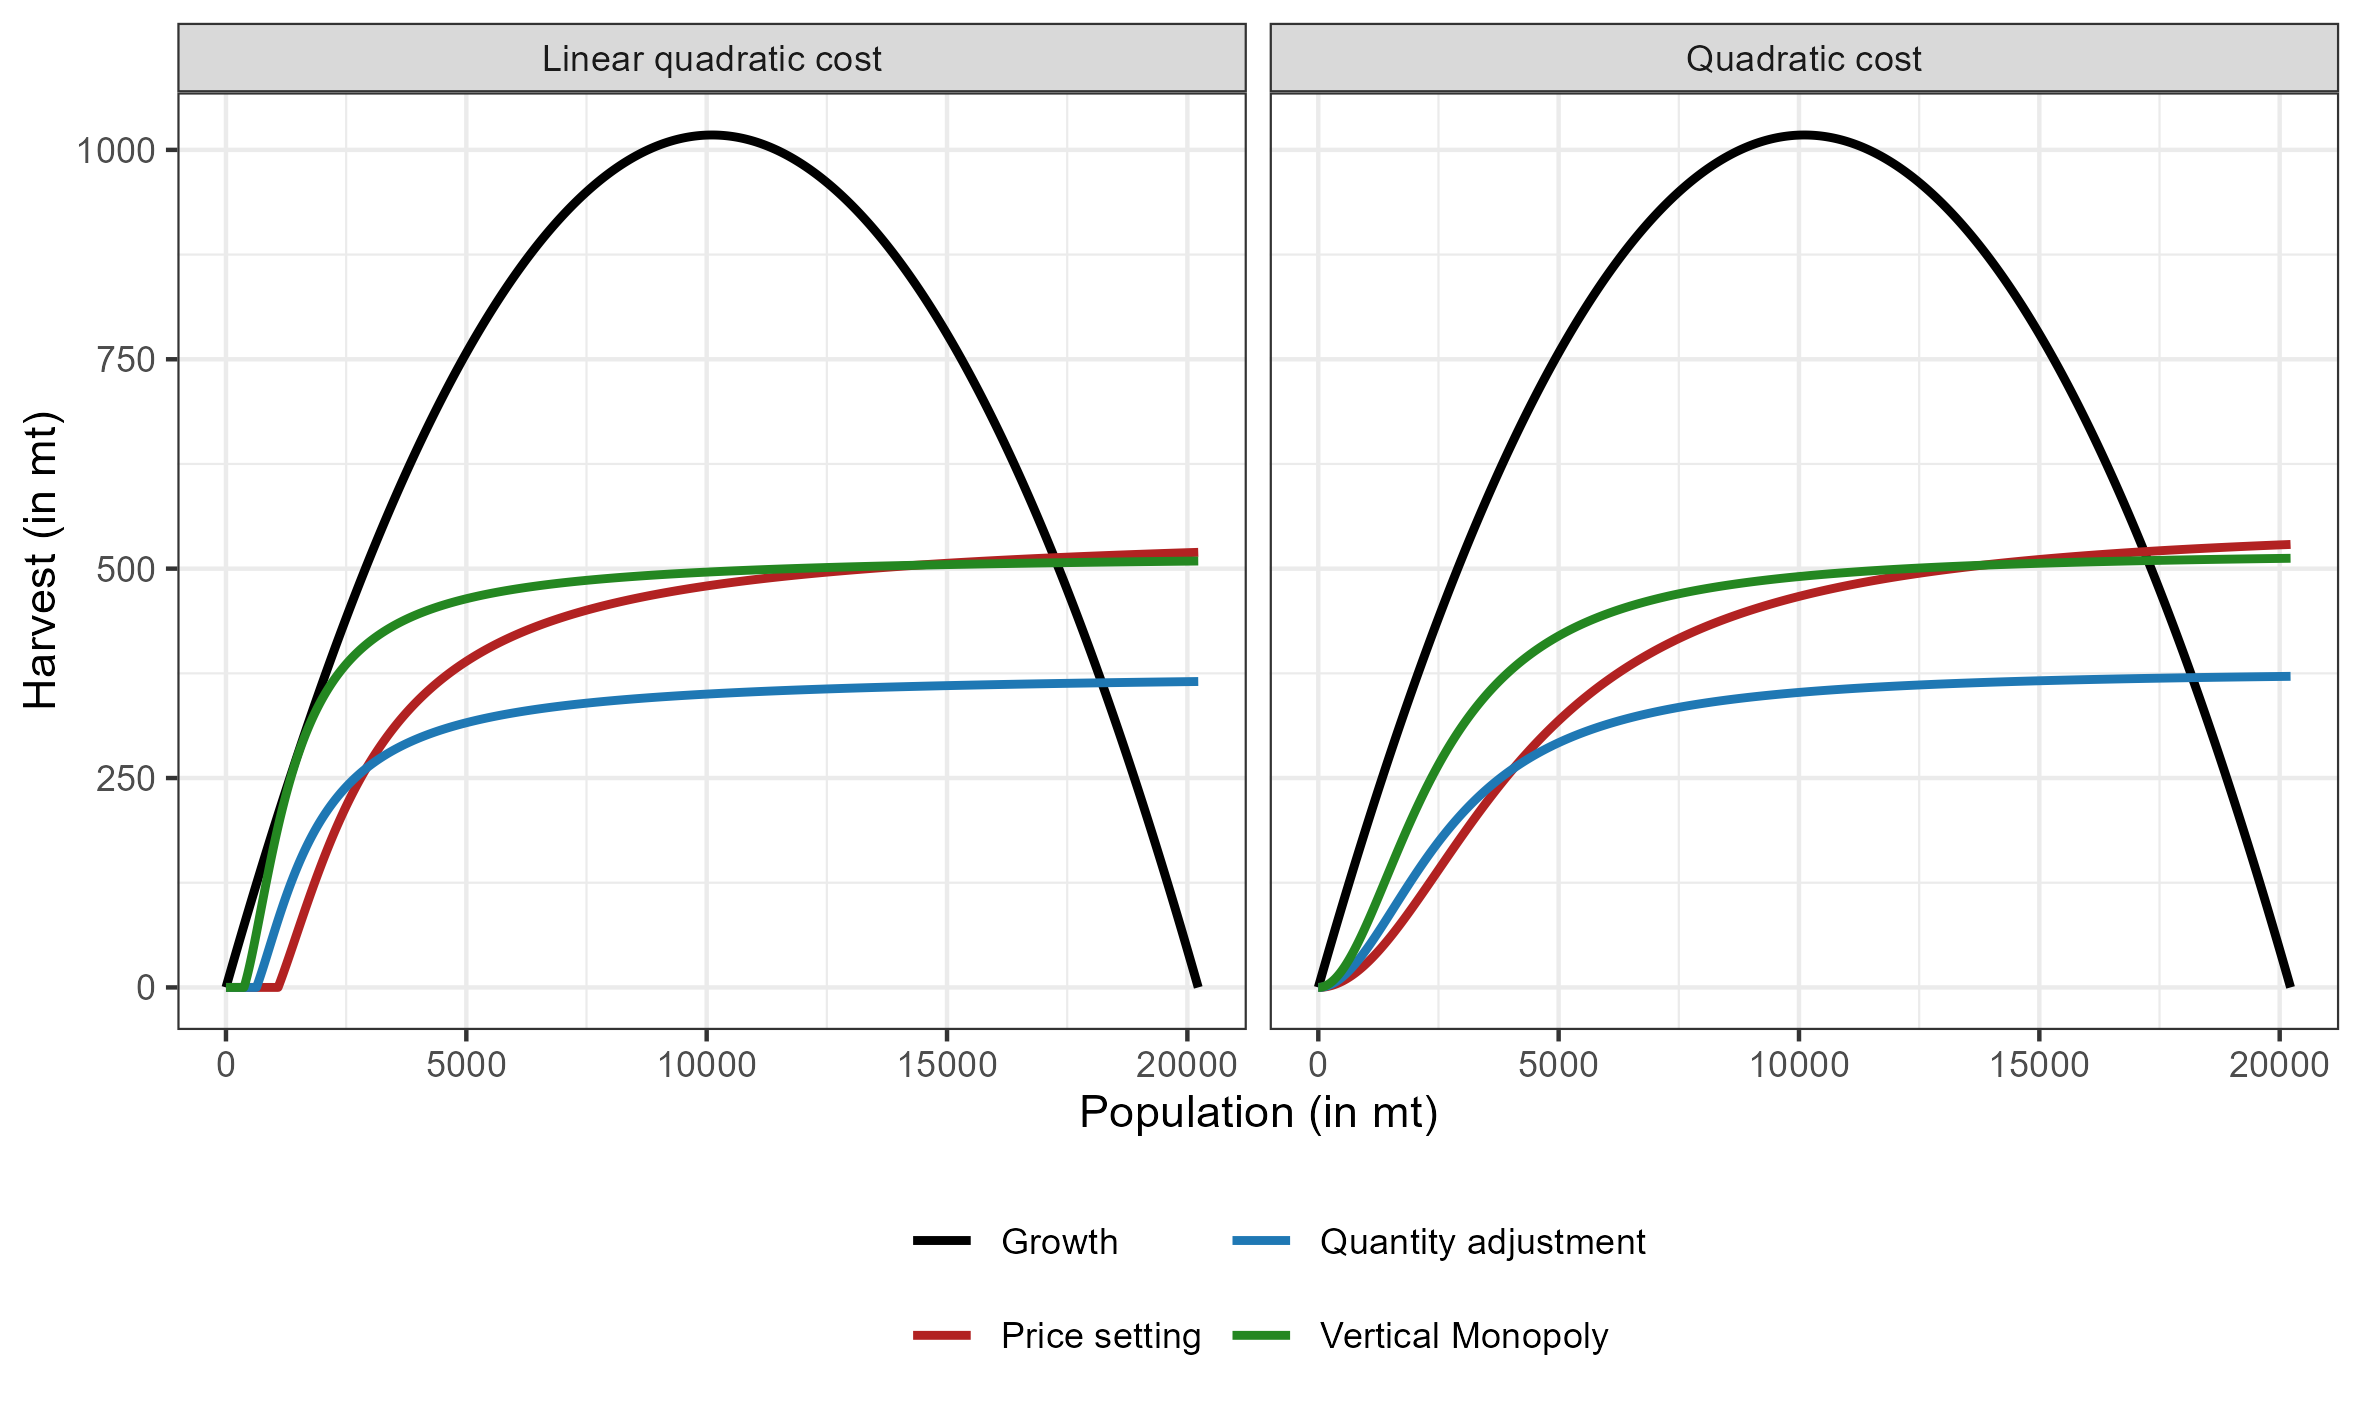
\includegraphics[width=\linewidth]{figures/Figure3.jpg}
%    \caption{Competition can be detrimental} %\label{fig:bertrand_bad}
%    \end{subfigure}

%    \vspace{1cm}
    
%    \begin{subfigure}[t]{0.45\textwidth}
%    \centering
%        \includegraphics[width=\linewidth]{figures/Figure3c.jpg} 
%        \caption{Counterintuitive equilibrium} \label{fig:counterint}
%    \end{subfigure}
    
%    \caption{Location of equilibria }
%   \label{fig:enter-label}
%\end{figure}
\subsection{Extensions}
\subsubsection{An oligopoly model}
We extend our model to gauge the impact of the number of traders and farmers. We denote by $\mathcal{I}$ the set of individual traders $i \in \mathcal{I}$ and by $\mathcal{J}$ the set of individual farmers $j \in \mathcal{J}$. The demand functions are : 
\begin{align}
    P_k^W &= \alpha^W - \beta^W \sum_{i \in \mathcal{I}}q^W_i - \gamma \sum_{j \in \mathcal{J}}q^F_j
    \\
    P_l^F &= \alpha^F - \beta^F \sum_{j \in \mathcal{J}}q^F_j - \gamma \sum_{i \in \mathcal{I}}q^W_i
\end{align}
\paragraph{Cournot oligopoly}
Each farmer and trader maximizes profits by taking as given its competitors' quantity commitments. We assume traders and farmers are homogeneous, i.e for each type of producer, costs are identical : 
\begin{align*}
    i,j \in \mathcal{I}, i\neq j, c_i = c_j = c\\
    k,l \in \mathcal{J}, k\neq l, v_k = v_l = v
\end{align*}
Assuming that $card(\mathcal{I}) = N$ and $card(\mathcal{J})=M$, the profit functions for each farmer and trader can be written as : 
\begin{align}
    \Pi_i^W &= \left(\alpha^W - \beta^W (N-1)q^W_{\Bar{i}} - \beta^W q_i^W - \gamma Mq^F - s - c \right)q_i^W\\
    \Pi_k^F &= \left(\alpha^F - \beta^F (M-1)q^F_{\Bar{k}} - \beta^F q_k^F - \gamma Nq^W - v \right)q_k^F
\end{align}
Where $q^W_{\Bar{i}}$ denotes the quantities sold by all other traders different from trader $k$ (and $q^F_{\Bar{i}}$ for farmers different from farmer $l$). 
Given that all players in each type are identical cost-wise, the reaction functions are : 
\begin{align}
   \forall i,j \in \mathcal{I}: q^W_i = q^W_j = q^W = \frac{\alpha^W - (s+c) - \gamma M q^F}{(N+1)\beta^W}\\
    \forall k,l \in \mathcal{J} : q^F_k = q^F_l = q^F = \frac{\alpha^F - v - \gamma N q^W}{(M+1)\beta^F}
\end{align}
The \textbf{Cournot-Nash equilibrium} is :
\begin{align}
    \text{Poaching : }q^W_{Cournot} &= \frac{\beta^F (M+1)(\alpha^W - (s+c)) - \gamma M (\alpha^F-v)}{\beta^W \beta^F (M+1)(N+1) - \gamma^2 NM}\\
    \text{Farming : } q^F_{Cournot} &= \frac{\beta^W (N+1) (\alpha^F-v) - \gamma N (\alpha^W - (s+c))}{\beta^W \beta^F (M+1)(N+1) - \gamma^2 NM}\\
\end{align}
%
The primary market (between poachers and traders) must clear, and $s(x)$ equates supply and demand: 
\begin{align}
    &Nq^W_{Cournot} = q^W \\
    \iff & s^{C^*}(x) = \frac{2W_2N\left[\beta^F (M+1) (\alpha^W-c) - \gamma M (\alpha^F - v)\right] + W_1 \sigma x (\beta^F \beta^W (M+1)(N+1) - \gamma^2 NM)}{\sigma^2 x^2 [\beta^F \beta^W (M+1) (N+1) - \gamma^2 NM] + 2W_2N(M+1)\beta^F}
\end{align}
%
Solving for the equilibrium quantity, the quantity supplied on the market by individual traders is : 
%
\begin{equation}
    q^W_{Cournot} = \frac{\sigma^2 x^2 \left[ \beta^F(M+1) (\alpha^W - c) - \gamma M(\alpha^F -v) \right] - \sigma x W_1 N(M+1) \beta^F}{\sigma^2 x^2 (\beta^F \beta^W (M+1)(N+1)-\gamma^2 NM) + 2W_2N(M+1)\beta^F}
\end{equation}
In our case study, when $c=0$, it 
shows that when the number of farmers is larger than the number of traders, the introduction of farming generates larger steady-state stocks. An interesting perspective is when there remains 1 sole trader, and the number of farmers increases: in this case, poaching is drastically cut down, as shown in Figure \ref{fig:cournot_oligo}.
%
When the number of traders is larger than the number of farmers, steady-state stocks decrease. In our context, when the number of traders is limited, increasing the number of farming facilities is a safe way to guarantee conservation outcomes. 

\begin{figure}[H]
    \centering
    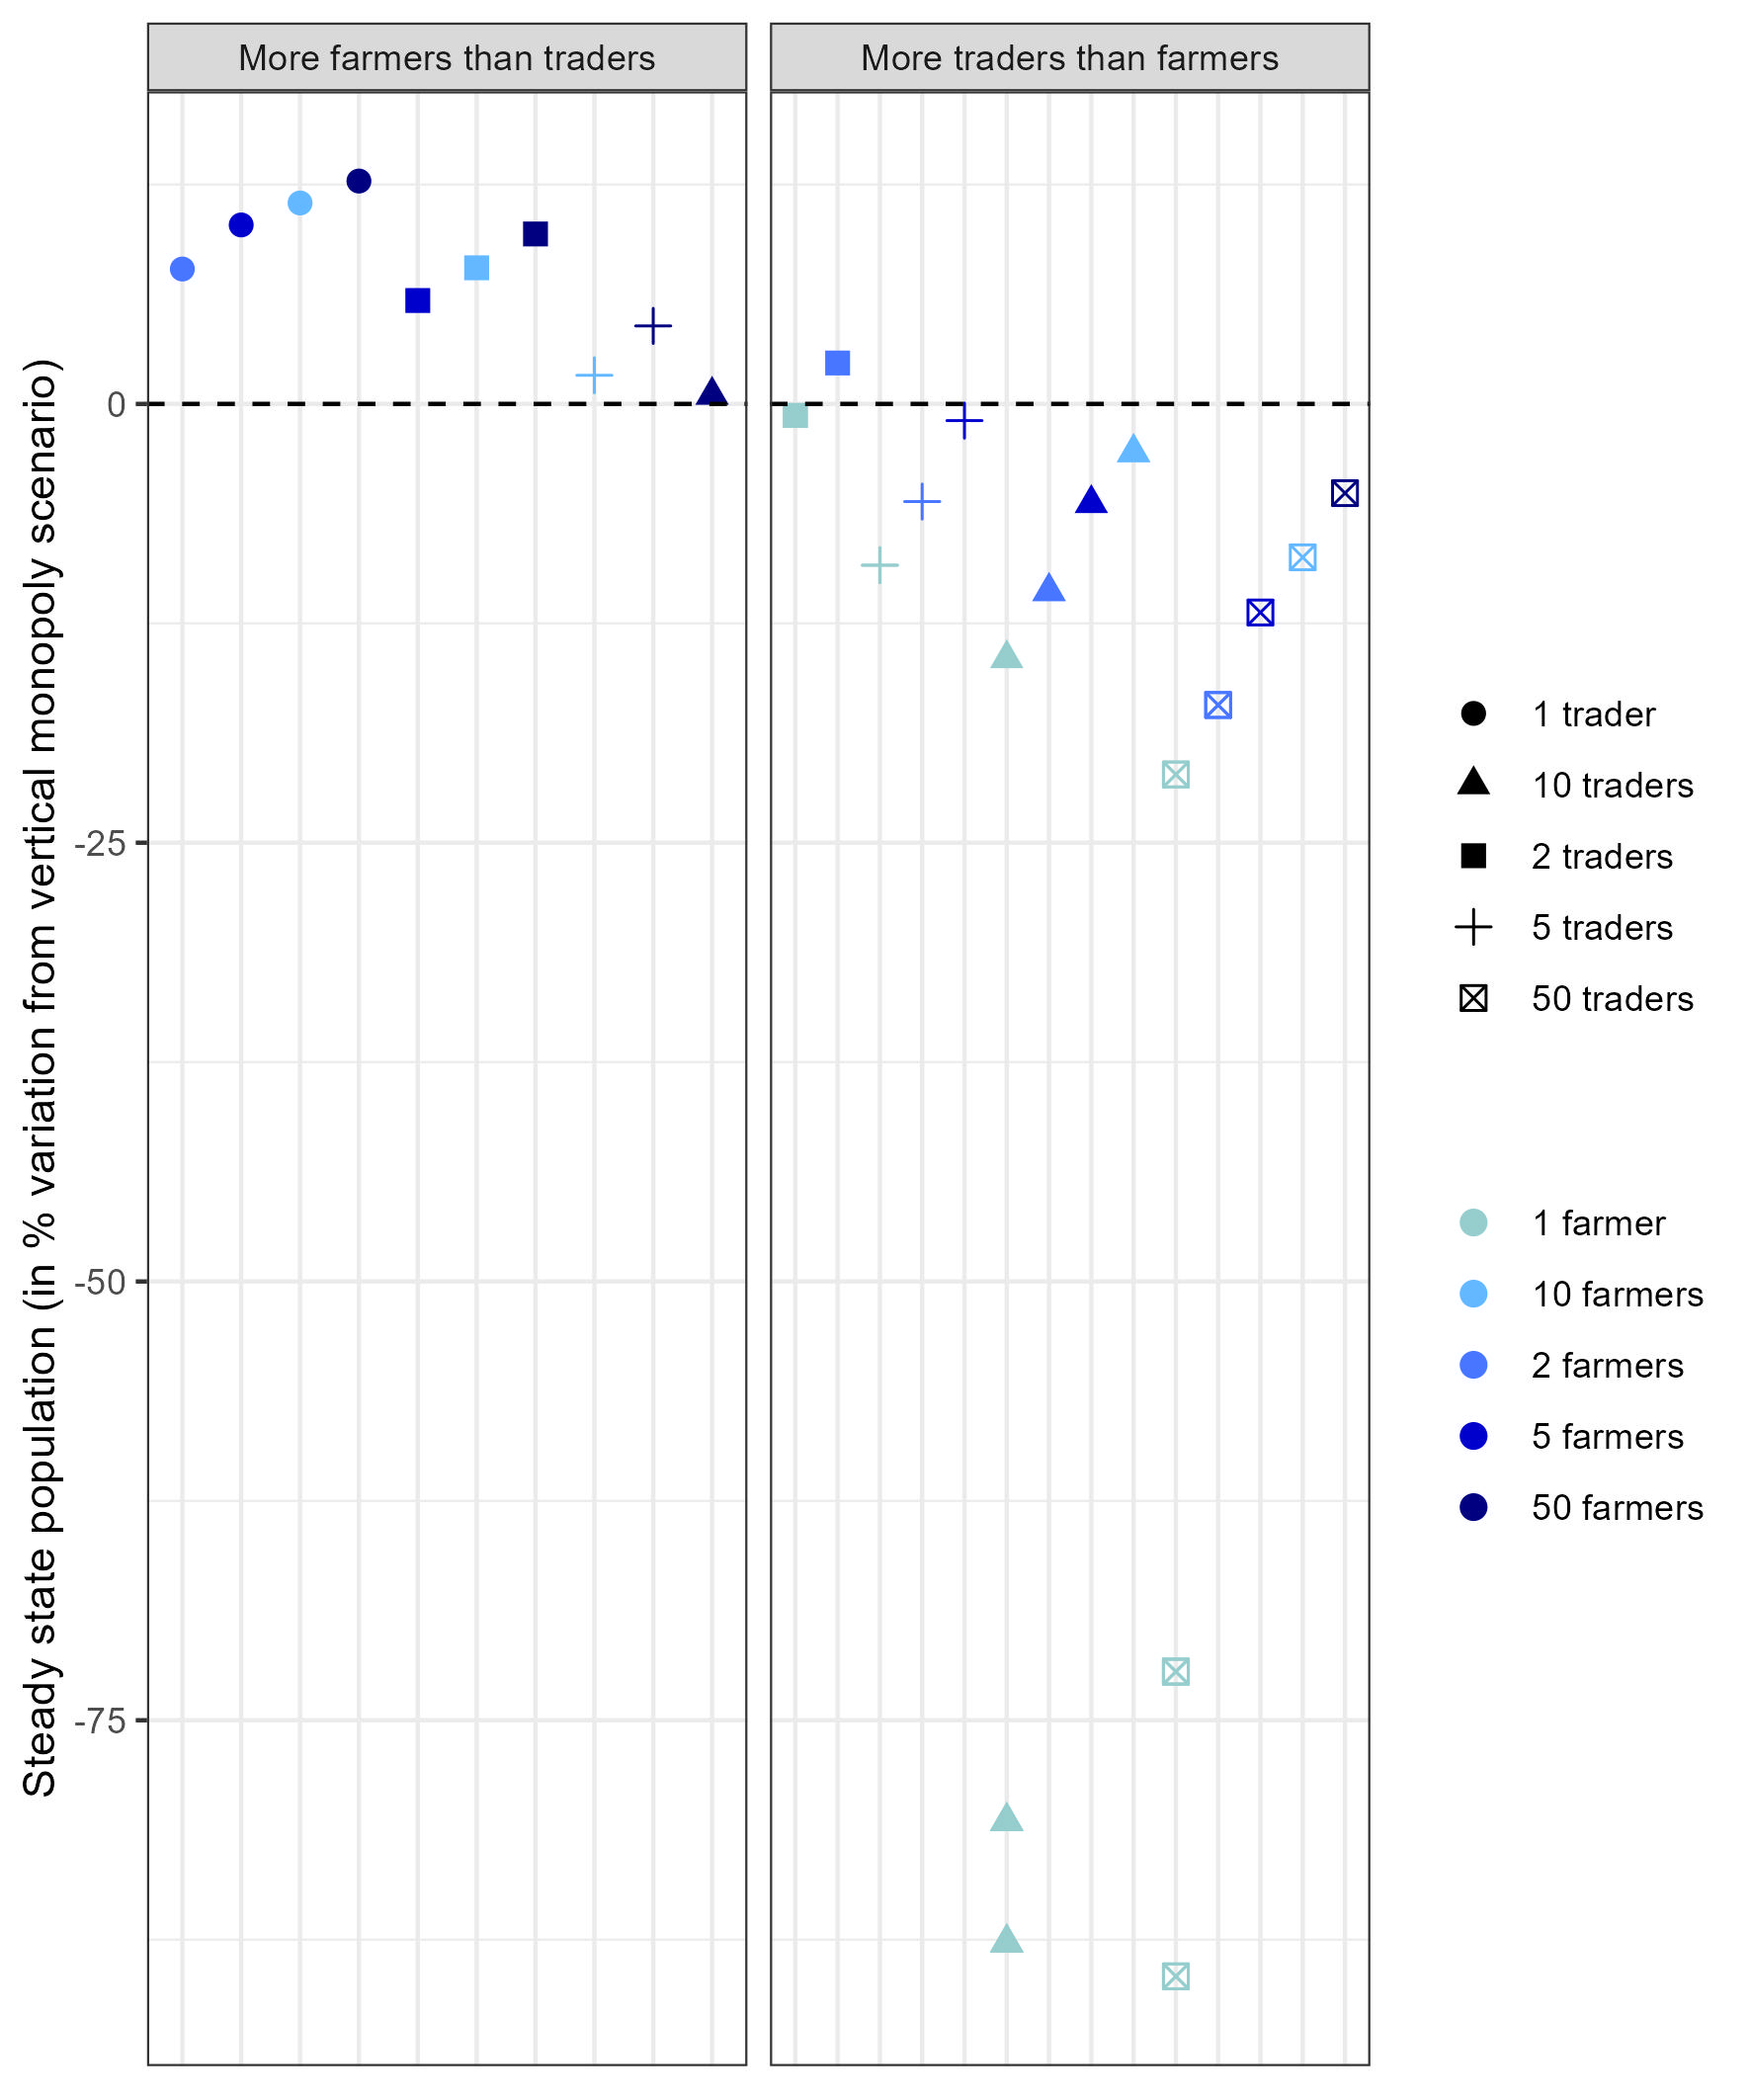
\includegraphics[width=.7\textwidth]{figures/totoaba/sup_figure1.jpg}
    \caption{Steady state outcomes when multiple traders and multiple farmers are  considered (an oligopoly) in the quantity adjustment scenario.}
    \subcaption*{ The left panel shows the steady state of the wild \textit{Totoaba macdonaldi} population when there are more farmers than traders. The right panel shows the steady state of the wild population when there are more traders than farmers}
    \label{fig:cournot_oligo}
\end{figure}
%
\paragraph{Bertrand oligopoly}
Using the same notations as previously, the demand functions can be written as : 
\begin{align}
    \forall i\in \mathcal{I} : q^W_i = q^W = \frac{1}{N}(a^W - b^W P^W - e P^F)\\
    \forall j \in \mathcal{J} : q^F_j = q^F = \frac{1}{M}(a^F - b^F P^F - e P^W)
\end{align}
Using these demand functions and solving for the reaction functions in each case yields : 
\begin{align}
    r^F(P^W) &= \frac{a^F + b^F v + eP^W}{2b^F}\\
    r^W(P^F) &= \frac{a^W + b^W (s+c) + e P^F}{2b^W}
\end{align}
These reaction functions are the same as in the duopoly case (see eq. \ref{eq:rf_bertrand}). This result shows that aggregate production is invariant to the number of farmers or traders as long as both are present on the market. Moreover, the individual production for traders is $\frac{1}{N} q^W_B$ and $\frac{1}{M}q^F_B$ with $q^W_B$ and $q^F_B$ referring to the duopoly equilibrium quantities for poached and farmed productions. In a Bertrand equilibrium, irrespective of the number of players, price-setting competition pushes the price to its minimum such that both firms still operate (given that traders have a stock-dependent production cost). Increased competition in the form of more players cannot push the prices further down. Therefore, aggregate output remains the same and individual production is divided among players. \\
This result further contradicts the results in \cite{damania_economics_2007}, as the authors find that increasing the number of players in a Bertrand set-up has detrimental effects on the steady-state stock. We find no effect, consistent with the theory and intuition. 
%
\subsubsection{Trader take over of the aquaculture sector}
%
In this section, we look at the 'extended cartel' scenario, where the vertical monopoly takes over the ownership of the aquaculture firm. \\
To gain intuition, assume poached and farmed products are perfect substitutes. On the one hand, the vertical monopoly has two production technologies:  poaching ( with a variable marginal cost, as the price paid to poachers depends on the population stock) and farming ( with a constant marginal cost). In this case, the vertical monopoly equates the marginal costs across production units; that is, it buys a poached product to poachers up until the marginal cost of an extra poached unit equates to that of a farmed unit. In this case, if the marginal cost of farming is lower than market prices absent farming, then poaching goes down. Notice that the only way for traders to limit the price paid to poachers is to maintain a healthy stock. Therefore, the new equilibrium population stock is larger than the initial stock, and poaching is lower.

Now consider the case at stake, where products are imperfect substitutes. In this case, the extended cartel does not only equate marginal costs, as marginal revenues diverge across products. We use the following model to investigate the resulting equilibrium. Let the profit of the extended cartel be:

\begin{equation}
\Pi(q^F, q^W) = (\alpha^W - \beta^W q^W - \gamma q^F - (s+c))q^W + (\alpha^F - \beta^F q^F - \gamma q^W - v)q^F
\end{equation}

The extended cartel maximizes its profit with respect to the poached and farmed products. The poached production it sells on end markets is : 

\begin{equation}
q^W = \frac{\sigma^2 x^2 (\beta^F(\alpha^W -c) - \gamma (\alpha^F - v)) - W_1 \beta^F \sigma x }{2(\beta^F W + \sigma^2 x^2 (\beta^F \beta^W - \gamma^2)) }
\end{equation}

Figure \ref{fig:extended_cartel} shows that if the 'extended cartel' scenario arises, poaching goes down, and the steady-state population increases.
%
\begin{figure}
    \centering
    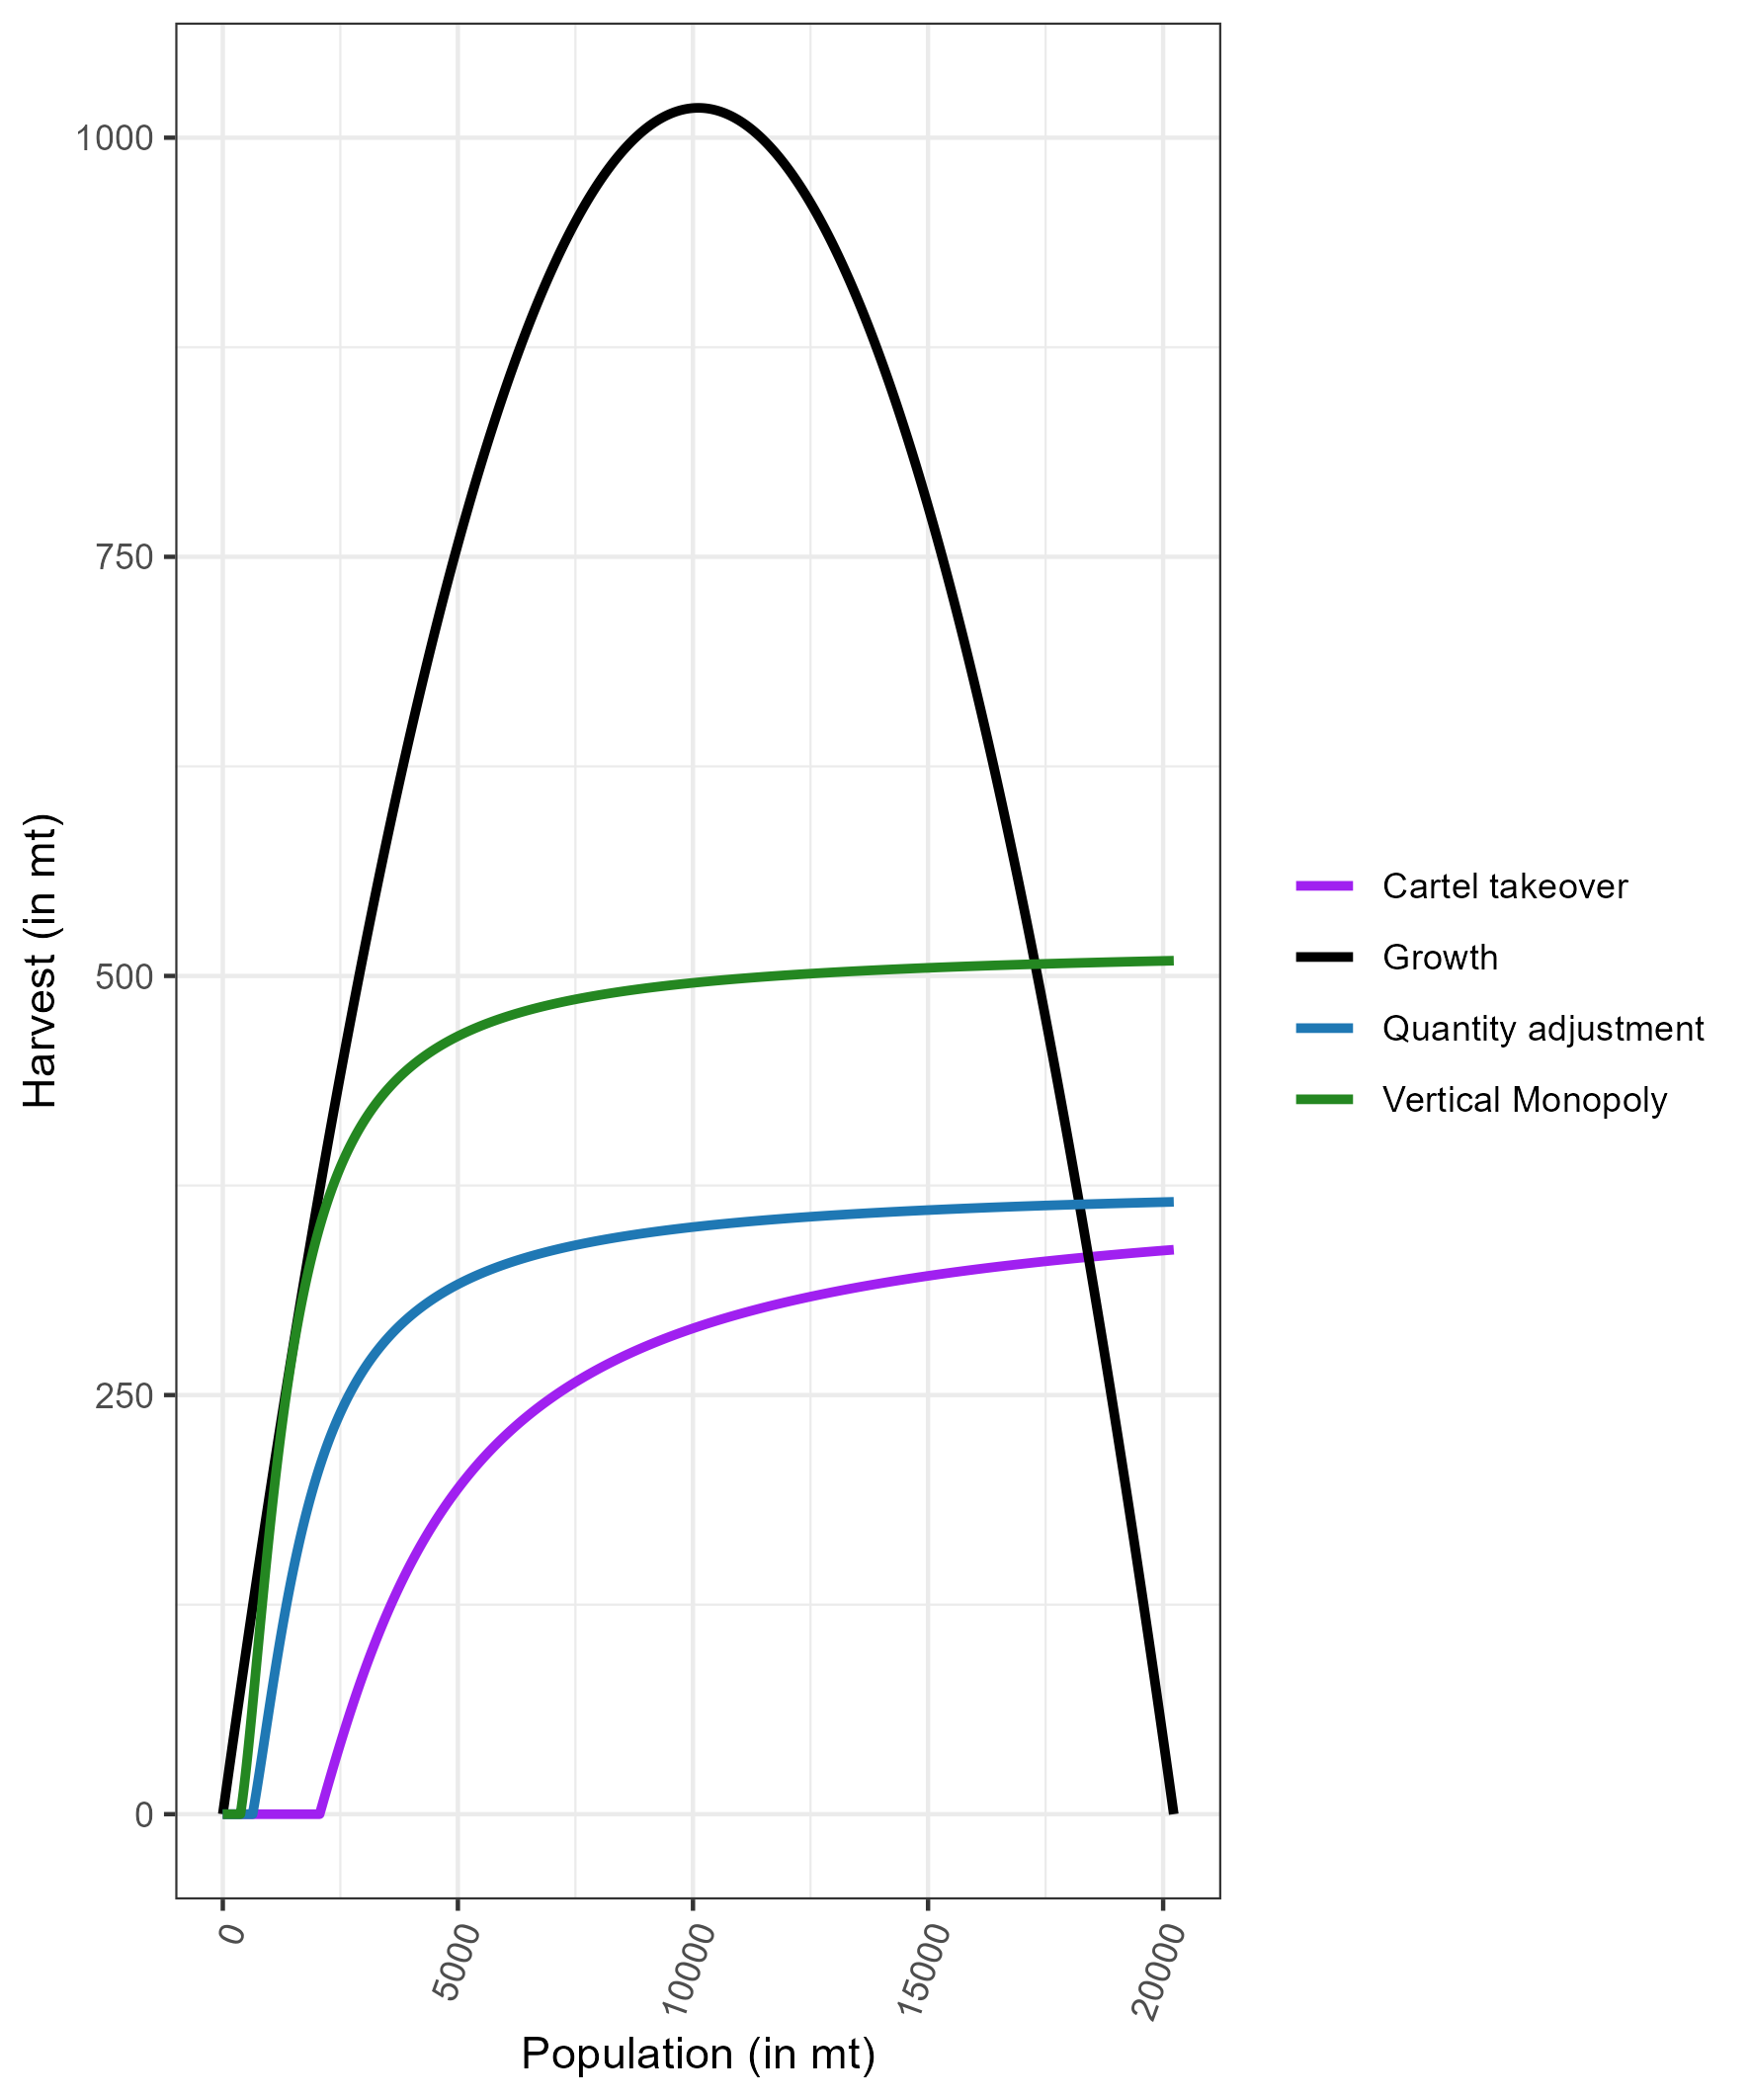
\includegraphics[width = .7\textwidth]{figures/totoaba/sup_figure2.png}
    \caption{ Steady-state equilibrium for the wild stock of \textit{Totoaba macdonaldi }in the ‘extended cartel’ scenario, where the vertical monopoly takes over the ownership of farming operations}
    \label{fig:extended_cartel}
\end{figure}

\subsection{Appendices}
\label{subsection:appendix_toto}
\subsubsection{Lemma 1 : content and proof}
\label{section:AppendixB}

Assume $\alpha^W = \alpha^m$ and $\beta^m  =\beta^W$, i.e., that the demand faced by the monopolist is the same as in the duopolistic case.  Comparing monopoly and Cournot harvest functions:
\begin{align*}
q^W_m &\geq q^W_c\\
    \Rightarrow v & \leq \Bar{v}=\alpha^F - \frac{\gamma(\alpha^m - c)\sigma^2x^2 - W_1\sigma x}{2\beta^m\sigma^2x^2 + 2W}
\end{align*}
First, look at when $x \to 0$ : 
$$
\lim_{x\to 0}\Bar{v} = \alpha^F
$$
This requires that farming costs are lower than the choke price for consumers on their market. This condition is necessary for a farm competitor to enter the market. 
\\
Second, acknowledge that the second part of the equation is weakly decreasing, but non-increasing. Assuming the carrying capacity goes to infinity, it is limited by :
$$
\lim_{x \to \infty}\Bar{v} = \alpha^F - \gamma\frac{(\alpha^m - c)}{2\beta^m}
$$
As fish abundance increases, the price paid to poachers decreases, as there is less scarcity. From equation (\ref{eq:price_poachers_cournot}), when $x \to \infty$, the price paid to poachers drops to 0. 
Moreover, notice that the last term in parenthesis is equation (\ref{eq:monop}) for $s=0$. Therefore, it means that the residual willingness to pay, when the poachers behave like a monopoly and $x\to \infty$, is larger than the unit cost of farming. 

If the market is truly duopolistic, in the sense that the poachers could not manage the stock such that they depress demand so much as to kick their competitor out of the market, then Cournot competition unambiguously leads to lower poaching levels than a monopoly does.
%
\subsubsection{Lemma 2}
\label{section:AppendixC}
Assume that the demand parameters are unchanged by the introduction of farmed substitutes, that is to say $\alpha^W  = \alpha ^m$ and $\beta^W= \beta^m$, and use the definition of the coefficients for the direct demand function:
\begin{align*}
 a^{j} &= \frac{\alpha^{j} \beta^{i} - \alpha^{i}\gamma}{\beta^{j} \beta^{i} - \gamma^2}; \hspace*{1cm}
  b^{j} = \frac{\beta^{i}}{\beta^{j} \beta^{i} - \gamma^2}\\
 a^m &= \frac{\alpha^m}{\beta^m}; \hspace*{2cm}
b^m = \frac{1}{\beta^m}
\end{align*}
For $i,j \in \{W, F\}$ and $m$ the monopoly case.
To establish Lemma 2, we compare $q^W_B$ and $q^W_m$. Equation (\ref{eq:harvest_monop}) can be rewritten as : 
$$
q^m(a^m, b^m) = \frac{\sigma^2 x^2(a^m - b^m c) - b^m W_1 \sigma x}{2\sigma^2 x^2 +2Wb^W}
$$
%
Therefore:
\begin{align*}
    &q^W_m \geq q_B^W\\
    \Rightarrow & v \leq \frac{a^m - b^m c}{b^Wb^Fe}\left[ \frac{2 W_2 b^W(2b^Fb^W - e^2) + (4b^Fb^W - e^2)\sigma^2 x^2}{2 \sigma^2 x^2 + 2 b^m W_2}\right]  - \frac{W_1 \sigma x[(4 b^F b^W - e^2)(b^m - b^W) + e^2 b^W]}{b^wb^Fe(2\sigma^2 x^2 + 2b^m W_2)} \\
    & - \frac{ea^F + c(e^2 - 2b^Wb^F) + 2b^F a^W}{b^F e}
\end{align*}
Notice that this equation can be reframed as : 
\begin{align*}
    F(x|c) \geq v \text{ where } F(x|c) = \Phi \frac{\eta + \mu x^2}{\theta + \nu x^2} -\frac{ \kappa x}{\omega x^2 + \epsilon} - \zeta
\end{align*}
And :
\begin{align*}
    &\Phi = \frac{a^m - b^mc}{b^W b^F e},\text{ }
    \eta = 2W_2b^W(2b^Wb^F - e^2),\text{ } 
    \mu = (4b^Wb^F - e^2)\sigma^2,\text{ }\\
    &\theta= 2W_2b^m,\text{ }
    \nu = 2\sigma^2,\text{ }
    \zeta  = (ea^F + c(e^2 - 2b^W b^F) + 2b^F a^W)\\
    \\
    &\kappa = \frac{W_1 \sigma [(4b^F b^W - e^2)(b^m - b^W) + e^2 b^W)]}{b^F*e}, \\
    &\text{ }\omega = 2b^Wb^Fe \sigma^2
    \text{ and } \epsilon = 2b^m b^W b^F e W_2
\end{align*}
\paragraph{Analysis of $\Phi \frac{\eta + \mu x^2}{\theta + \nu x^2}$:} if $\mu \theta - \nu \eta<0$, the first component of $F(x|c)$ is decreasing:
\begin{align*}
&(4b^Wb^F - e^2)b^m -2(b^Wb^F-e^2)b^W<0\\
\iff & \frac{\gamma^2}{\beta^m (\beta^W\beta^F - \gamma^2)^3}\left[ \beta^m \beta^F + \gamma^2 -4\beta^F \beta^W \right]<0\\
\end{align*}
Under the assumption that $\beta^m = \beta^W = \beta^F = \beta$, it is clear that 
$$
\frac{\gamma^2}{\beta(\beta^2 - \gamma^2)}(\gamma^2 - 3 \beta^2) <0
$$
as $\gamma < \beta$. 
Therefore, $\Phi \frac{\eta + \mu x^2}{\theta + \nu x^2}$ is \textit{decreasing} $\forall x$
\paragraph{Analysis of $\frac{\kappa x}{\omega x^2 + \epsilon}$}: the second component of $F(x|c)$ is increasing for $x \leq \sqrt{\frac{\epsilon}{\omega}}$, and decreasing after, since $x\in \mathbb{R}^+$. Noticing that $\kappa <0$: 
\begin{itemize}
    \item For $x \in \left[0,\frac{1}{\sigma}\sqrt{W_2 b^m} \right]$, $\frac{\kappa x}{\omega x^2 + \epsilon}$ is negative and decreasing
    \item For $x>\frac{1}{\sigma}\sqrt{W_2 b^m}$, $\frac{\kappa x}{\omega x^2 + \epsilon}$ is negative and increasing
\end{itemize}

\paragraph{Conclusion}
Overall, $F(x|c)$ is such that : 
\begin{itemize}
    \item For $x \leq \frac{1}{\sigma}\sqrt{W_2 b^m}$, the first component is decreasing, while the second component is increasing
    \item For $x \geq \frac{1}{\sigma}\sqrt{W_2 b^m}$, the first component is decreasing and the second component is decreasing
\end{itemize}

Hence, $F(x|c)$ is bounded above by $\max \big(F(0|c),F(\frac{1}{\sigma}\sqrt{W_2 b^m}|c)\big)$, and bounded below by $F(K|c)$ where $K$ is the system carrying capacity. Therefore:
\begin{enumerate}
    \item If $v<F(K|c)$, then Bertrand harvest is always lower than monopoly harvest
    \item If $F(K|c)<v<F(0|c)$, then Bertrand harvest starts by being lower than in the monopoly case, but gets larger for large stock values. 
    \item Eventually, if $F(0|c)<v$, then Bertrand harvest is always larger than in the monopoly case
\end{enumerate}
Figure \ref{fig:lemma2} illustrates this lemma with our parameter specification.
\begin{figure}[h]
    \centering
    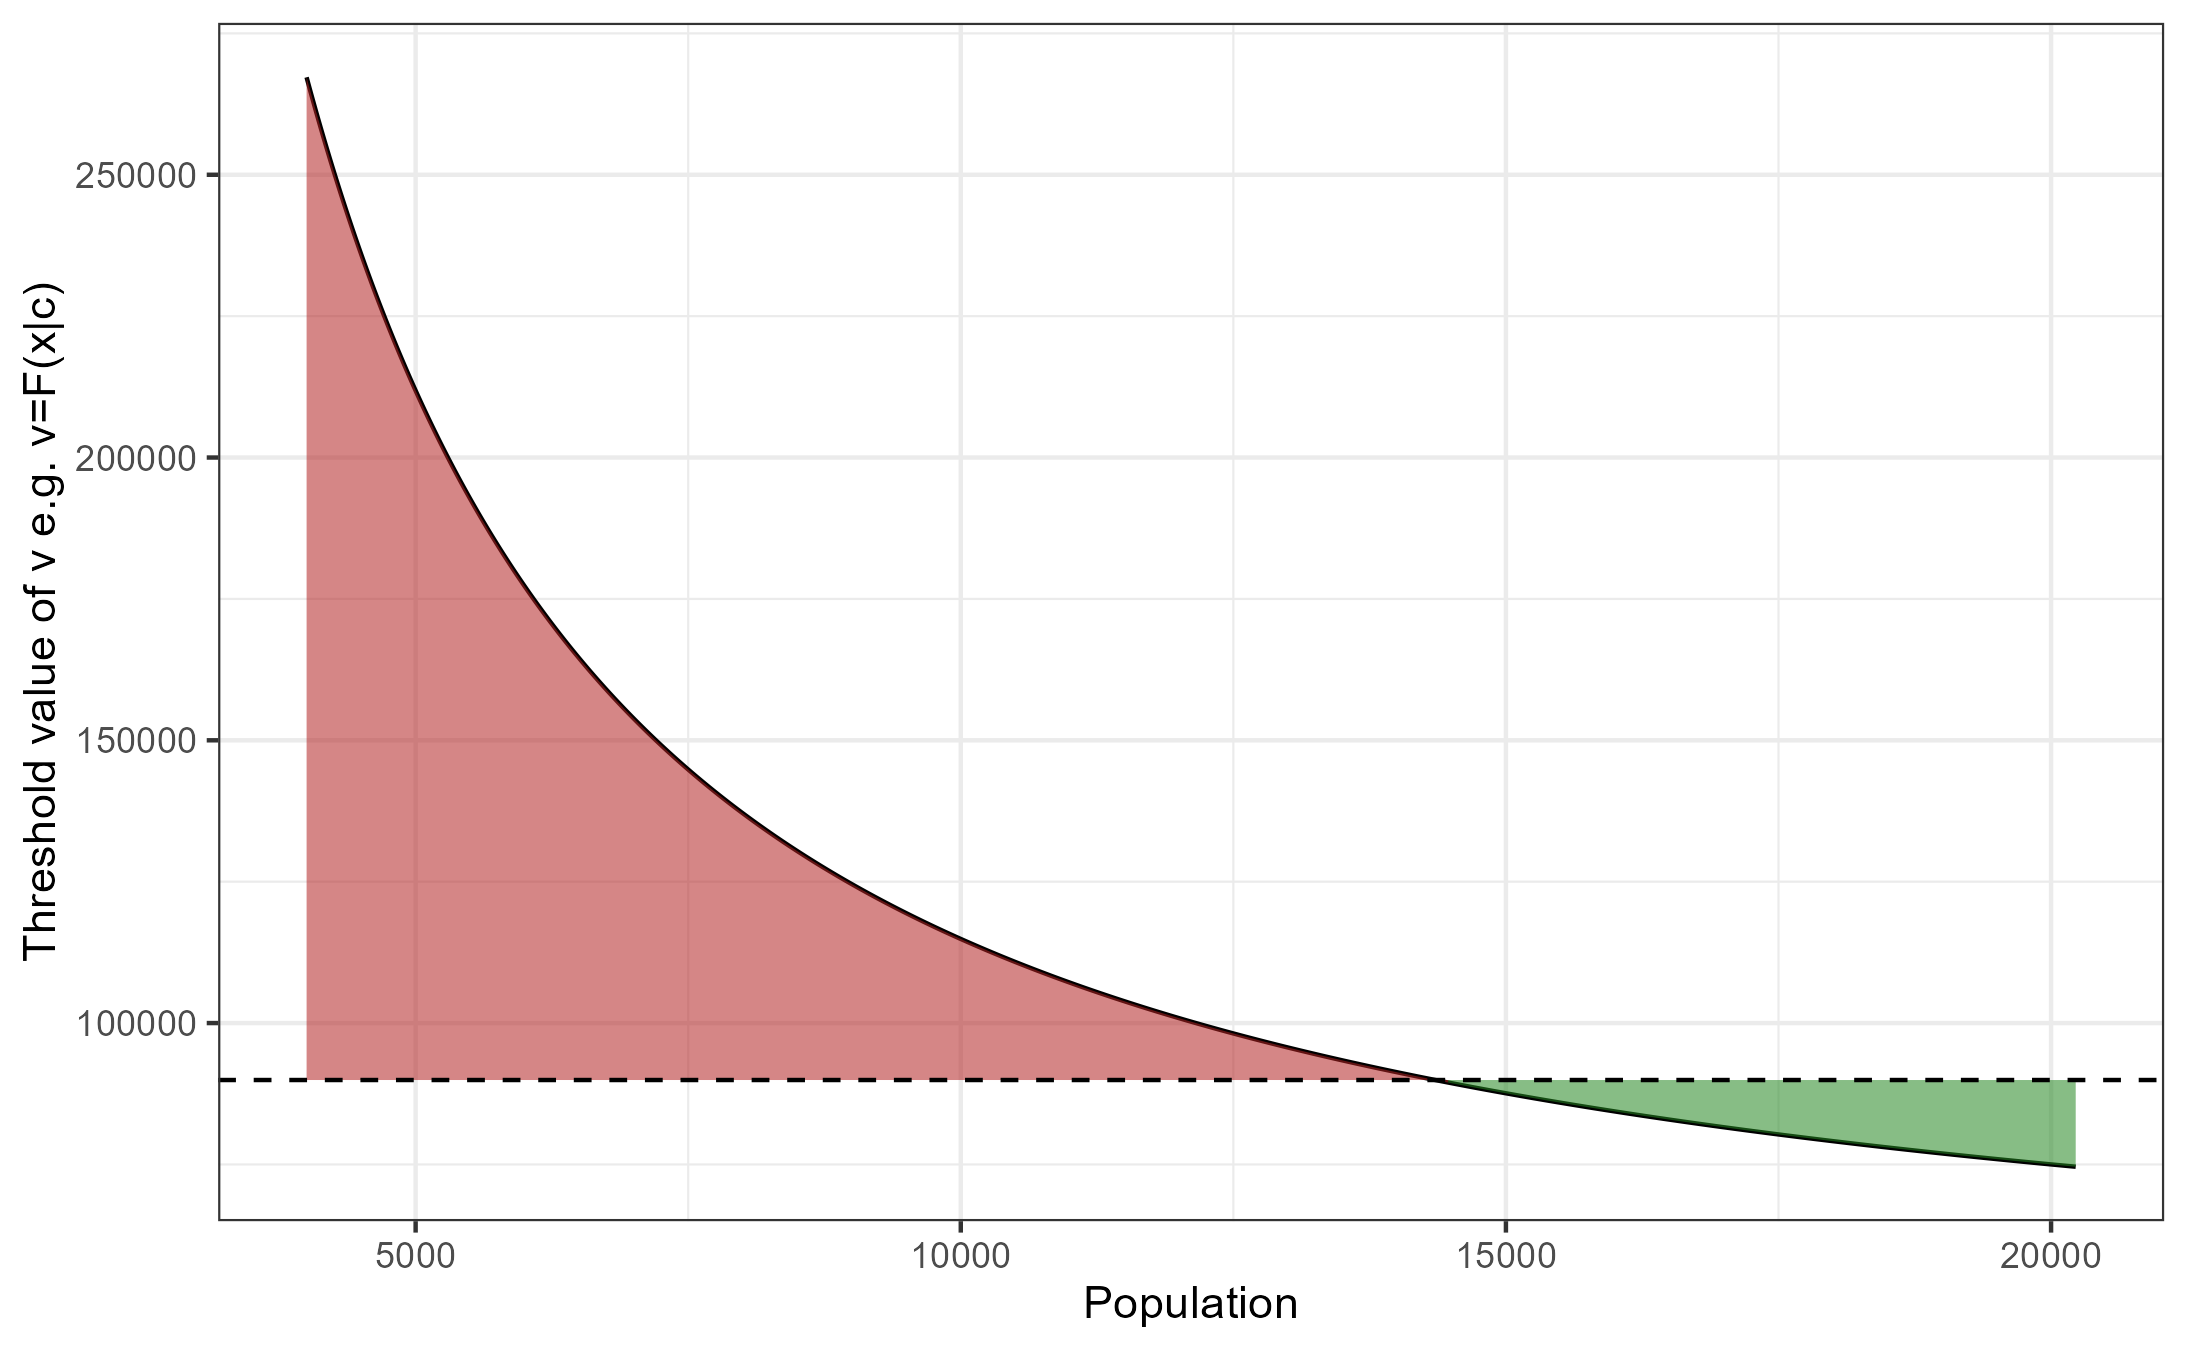
\includegraphics[width=0.8\linewidth]{figures/totoaba/lemma2_bertrand.png}
    \caption{Evolution of the threshold $v$ to compare vertical monopoly and price setting (Bertrand) harvest functions}
    \subcaption*{In green, vertical monopoly harvests more than in the price setting equilibrium. For larger population values, in red, price setting leads to more harvest than the vertical monopoly. This illustrates our main specification and property $2$ above.}
    \label{fig:lemma2}
\end{figure}

%Figure \ref{fig:bertrand_proof} illustrates this property. The top, red, dashed curve corresponds to case 1, where Bertrand always yields a larger harvest. For intermediary values, first, in the red-shaded area, Bertrand harvest is lower than in the monopoly case. For large stock values, however, it becomes larger than in the monopoly case, as displayed in the black-shaded area. Eventually, the bottom, black, dotted curve shows low values of $v$ where Bertrand harvest is always lower than in the monopoly case.

%\begin{figure}[H]
%    \centering
%    \includegraphics[width = .6\textwidth]{figures/Figure6_Lemma4_zoomed.jpg}
%    \caption{$F(x)$ and $v$ summarise when Bertrand harvest is larger or lower than in monopoly. In the red-shaded area, Bertrand harvest is lower than in the monopoly case. In the grey-shaded area, it is larger. }
%    \label{fig:bertrand_proof}
%\end{figure}

\paragraph{Corner equilibrium:}
for a corner solution to emerge, it must be that $q_B^{w*}=0$,
\begin{equation}
    v = v(x) = \frac{W_1(2b^F b^W - e^2)}{\sigma x b^F e} - \frac{2b^F a^W + ea^F + c(e^2 - 2b^W b^F)}{b^F e }
    \label{eq:v_corner}
\end{equation}
Equation \ref{eq:v_corner} shows that for low stock values, costs can still be positive and poaching disappear. However, to ensure that poaching is \textit{never} beneficial in the Bertrand equilibrium, it must be that $v = \min v(x) = - \frac{2b^F a^W + ea^F + c(e^2 - 2b^W b^F)}{b^F e v}$. In this case, the subsidy rate is so high that production is always beneficial for the farmer, and prices are too low for the trader to compete. In our baseline specification, this would amount to $v = - 720,855$ USD.  

%Figure \ref{fig:v_poaching_stop} shows the evolution of $v$ as substitutability and trading costs vary. 
%\begin{figure}[H]
%    \centering
%    \includegraphics[width = .8\textwidth]{figures/Figure7_v_poaching_stop.jpg}
%    \caption{$v$ for poaching to stop in a Bertrand equilibrium as a function of $\gamma$ and $c$}
%    \label{fig:v_poaching_stop}
%\end{figure}
%\subsubsection{Linear quadratic cost model}
%\label{sec:linear quadratic}

%In this section, we use a different cost specification for the fishery : 
%\begin{equation}
%    C(E) = W_1 E + W_2 \frac{E^2}{2}
%\end{equation}

%In this case, optimal effort is : 
%\begin{equation}
%    E^* = \frac{s\sigma x - W_1}{2W_2}
%\end{equation}
%And the quantity provided is : 
%\begin{equation}
%    q^W = \frac{s\sigma^2 x^2 - W_1 \sigma x}{2W_2} 
%\end{equation}

%\paragraph{In the vertical monopoly equilibrium,} demand from the monopoly does not change, but the supply does. 

%\begin{align}
%    \text{Price paid to poachers :} s^*_m(x) &= \frac{W_2 (\alpha_m -c) + \beta^m (W_1 \sigma x) }{ \sigma^2 x^2 \beta^m + W_2 }\\
%        \text{Poaching : } q^*_m(x) &=\frac{\sigma^2 x^2 (\alpha_m - c) - W_1 \sigma x}{2(\sigma^2 x^2 \beta^m +W_2)}
%\end{align}


%\paragraph{In the Cournot equilibrium, } demand remains unchanged, but supply is changed. 
%\begin{align}
%    \text{Price paid to poachers: } s_C^*(x) &= \frac{2 W_2(2\beta^F(\alpha_w - c) - \gamma(\alpha^m - v)) + W_1 \sigma x(4\beta^F\beta^W - \gamma^2)}{4W_2 \beta^F + \sigma^2 x^2(4\beta^F\beta^W -\gamma^2)} \\
%    \text{Poaching : } q^{C*}_W(x) &= \frac{\sigma^2 x^2(2\beta^F(\alpha^w -c) - \gamma(\alpha^F - v)) - 2\beta^F W_1 \sigma x}{4 W_2 \beta^F + \sigma^2 x^2(4\beta^W \beta^F - \gamma^2)}
%\end{align}

%\paragraph{In the Bertrand equilibrium }
%\begin{align}
%    \text{Price paid to poachers : } s_B^*(x) &=\frac{2 W_2 b^W[b^F(2a^w + ev) + e a_F + c(e^2 - 2b^Wb^F)] + W_1 \sigma x (4b^Fb^W - e^2)}{\sigma^2 x^2 (4b^F b^W - e^2) + 2 W_2 b^W(2b^F b^W - e^2)}
%\end{align}

%We use data collected at the vessel level to calibrate $W$ in the main specification and calibrate the marginal cost of effort to be equal to the observed average cost (the residual being a fixed cost parameter) in our data.

%Given that we have a 2 unknown equations for a single solution, a wide range of solutions for $W_1$ and $W_2$. Figure \ref{fig:equilibria_lq} shows the equilibria emerging from different $W_1$ and $W_2$ values. For specifications where the quadratic parameter $W_2$ is low, the \textit{vertical monopoly} can result in a drastic decline in steady-state population, while introducing aquaculture still yields substantial benefits in terms of steady-state population. For intermediate weights between the linear and quadratic parameters, results do not change drastically, and for large values of the quadratic parameter, results are not significantly different. Note that under the linear quadratic specification, low steady-state populations do not emerge in the price setting (Bertrand) equilibrium. 



\newpage
%\section{Supplementary data and empirical results}
%\subsection{Data}
%\subsubsection{Parameters for calibration}
%See table \ref{tab:params}.


%\subsubsection{Information about the cost of poaching}



%\subsubsection{Information about the cost of farming}
%See table \ref{tab:costv}


%\subsubsection{Demand estimation}
%See table \ref{tab:demand}


%\subsubsection{Individual growth curves for farmed versus wild totoaba, using the von Bertlaffery growth}
%See figure \ref{fig:vbgf}

%\subsection{Empirical results}

%\subsubsection{Impact of aquaculture on steady-state stock in different market structures}
%See table \ref{tab:oa_comp_aquaculture}

%\subsubsection{Impact of farming and transaction costs on equilibria}
%See figure \ref{fig:cost_equilibrium}.




%\subsubsection{Impact of demand variation and substitutability on steady state populations}
%Figure 4 (in manuscript) shows the evolution of steady-state populations in the market structures under study. The three different panels show results for values of $\gamma$ such that $\gamma \in \{ 0.1\beta, 0.5\beta, 0.9\beta \}$. 

%The three quadrants, delineated by dotted lines, display the type of equilibrium: the top panel is the high, stable state, the middle panel is the middle, unstable state, and the bottom panel is the low and stable state. Results show that the interaction between the expansion of demand and the substitutability of goods creates nontrivial results.

%First, in the monopoly case, increasing demand unambiguously leads to (i) the apparition of low, stable steady states (when $\alpha' >1.2 \alpha)$ and (ii) lower steady-state values. When farming is introduced, if demand increases, the effect of substitutability is key. 

%For low substitutability values,  competition increases the steady state values, compared to monopoly if it were to face increased demand.
%However, they yield significantly lower values than in the status quo equilibrium. When substitutability increases, and low stable steady states emerge. When substitutability increases ($\gamma = .5\beta$), Cournot competition can accomodate a 20\% increase in demand without harming the stock. If Bertrand equilibrium were to arise, it would result in a lower steady state equilibrium than the status quo equilibrium. The threat of low stable steady states emerges as well. When substitutability between products is large ($\gamma = .9\beta$), a Cournot outcome can accomodate a 40\% increase in demand, while population in a Bertrand equilibrium would be severely depleted. 

%Overall, substitutability has bifurcation values, changing the nature of the equilibria (1 equilibrium \textit{v.} 3 equilibria) as demand increases. When substitutability is large enough, demand can increase without changing the structure of the equilibria. 
%\newpage

%\section{Supplementary discussion and conclusion}


%Several assumptions underlie our results.

%First, we implicitly assume that the vertical monopoly does not discount future profits. Notwithstanding this polar assumption, economic theory shows that if profits are linear in effort, a monopolist owner of a renewable resource will lead to less effort, less catch and a larger population at a steady state, with a positive discount rate \citep{Crutchfield1962}

%Our set-up uses a fisher profit function that is quadratic in effort, and no discounting from the vertical monopoly. Simulations yield similar results. It is unclear how a positive discount rate would impact our conclusions (both in terms of existence and stability of the equilibrium) but our conclusions are robust to varying parameters that impact the ptimal response in a similar way.

%Second, we assume that farming rotations are invariant to market structure (following \cite{MITRA1986229}). However, existing results may be challenged as the model may be seen as artificially restrictive. In this case, they assume full replacement of the resource (i.e, when one fish is harvested, a new one has to spawn), as well as fixed production capacity (in their case, fixed land for forestry), and the life-span of a resource (i.e, they do not allow for a resource to go beyond a certain age). In doing so, they do not allow for adjusting production capacity nor how and when production reached the market. Further research is needed to actualize this result. 

%Third, we assume a linear demand model where quality does not play a role. In real life, there is a size/age premium for totoaba swim bladders. Our model takes the average quality as given. As the distribution of swim bladder size seems skewed to the left, aquaculture could operate on a luxury market and further displace demand. 


%Third, we assume that the cost structure of farming is linear, and does not depend on the wild population stock. However, as stocks plummet, security expenses are likely to increase\footnote{Famous examples include farming of rhinos, where security expenses skyrocketed as the rarity of rhino horns increased (see \url{https://www.cbsnews.com/news/rhino-farm-auction-john-hume-seeks-billionaire-to-carry-on-conservation-work/ })}. Therefore, costs may be quadratic in the stock. Eventually, the ecological requirement for farming and the corresponding location of the farming operation are important variables in limiting security expenses.
\newpage

\section*{Supplementary Figures and Tables}
\setcounter{table}{5}

\begin{figure}[H]
    \centering
    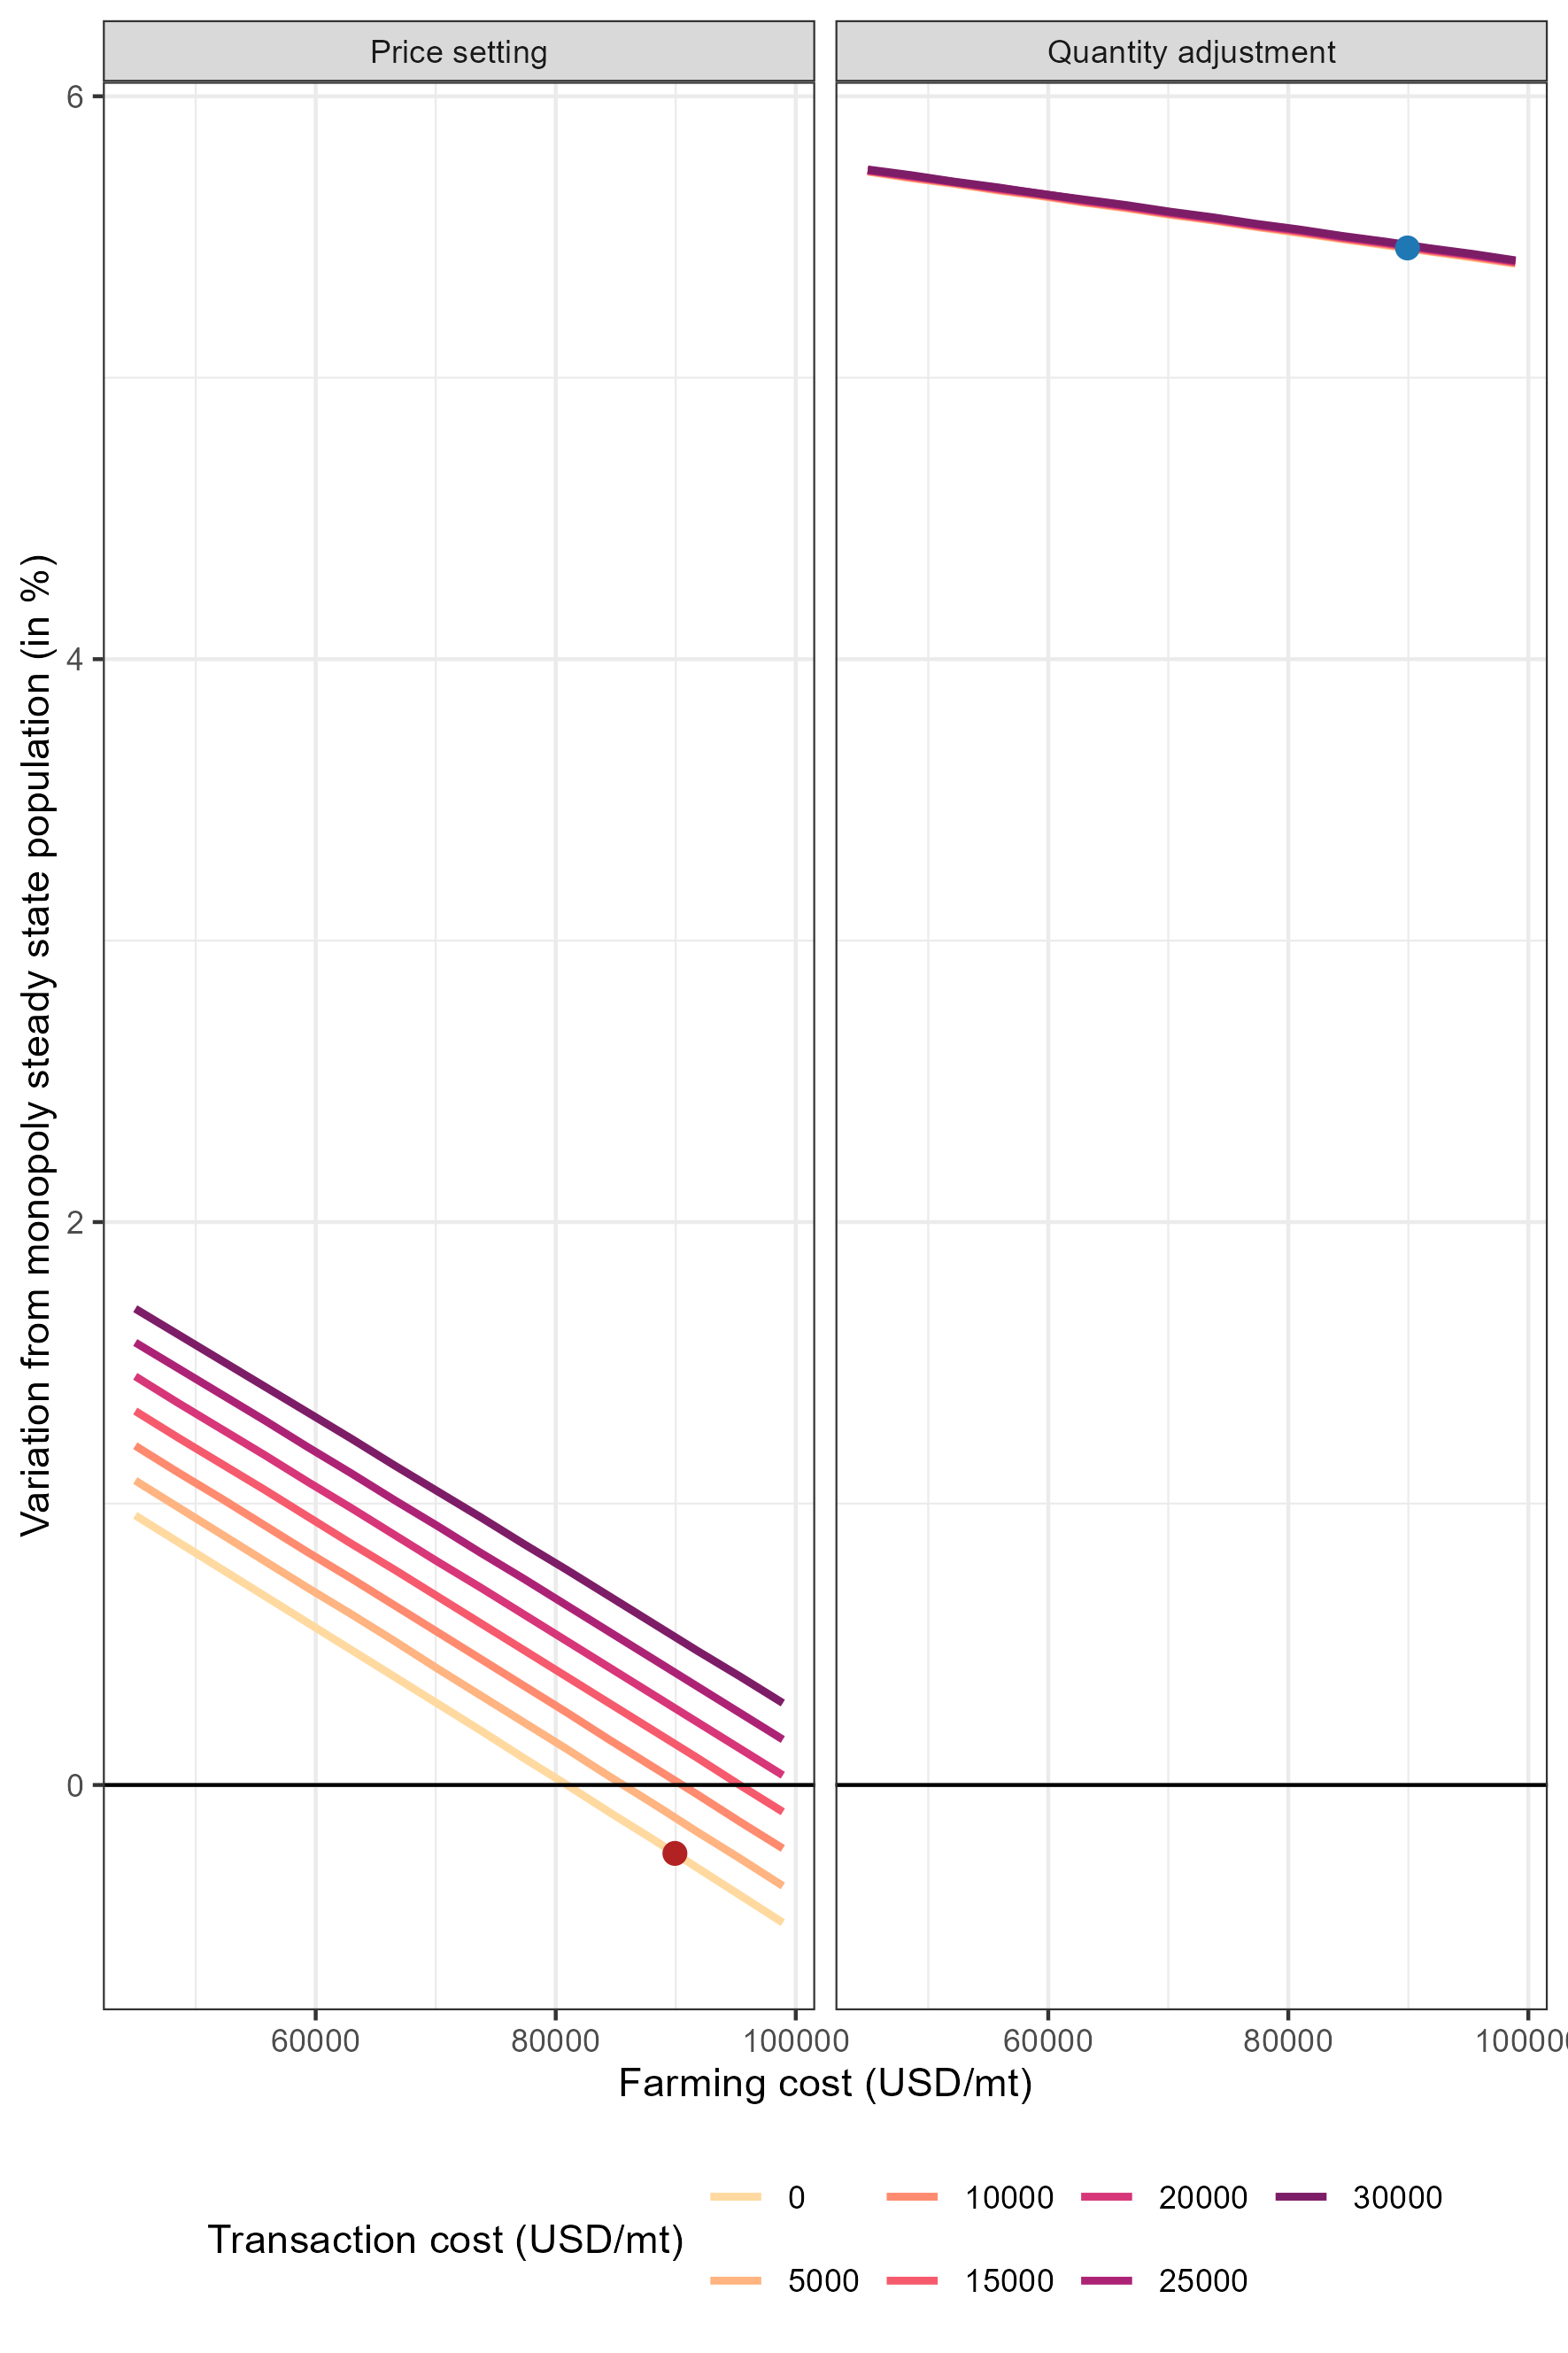
\includegraphics[width = .7\textwidth]{figures/totoaba/sup_figure3.png}
    \caption{Percent change in steady state population across scenarios, following the joint evolution of illegal transaction and farming costs}
    \subcaption*{Red and blue dots represent baseline results in the price setting and quantity adjustment scenarios}
    \label{fig:c_and_v}
\end{figure}
\newpage

%\setcounter{figure}{3}    

\begin{figure}[H]
    \centering
    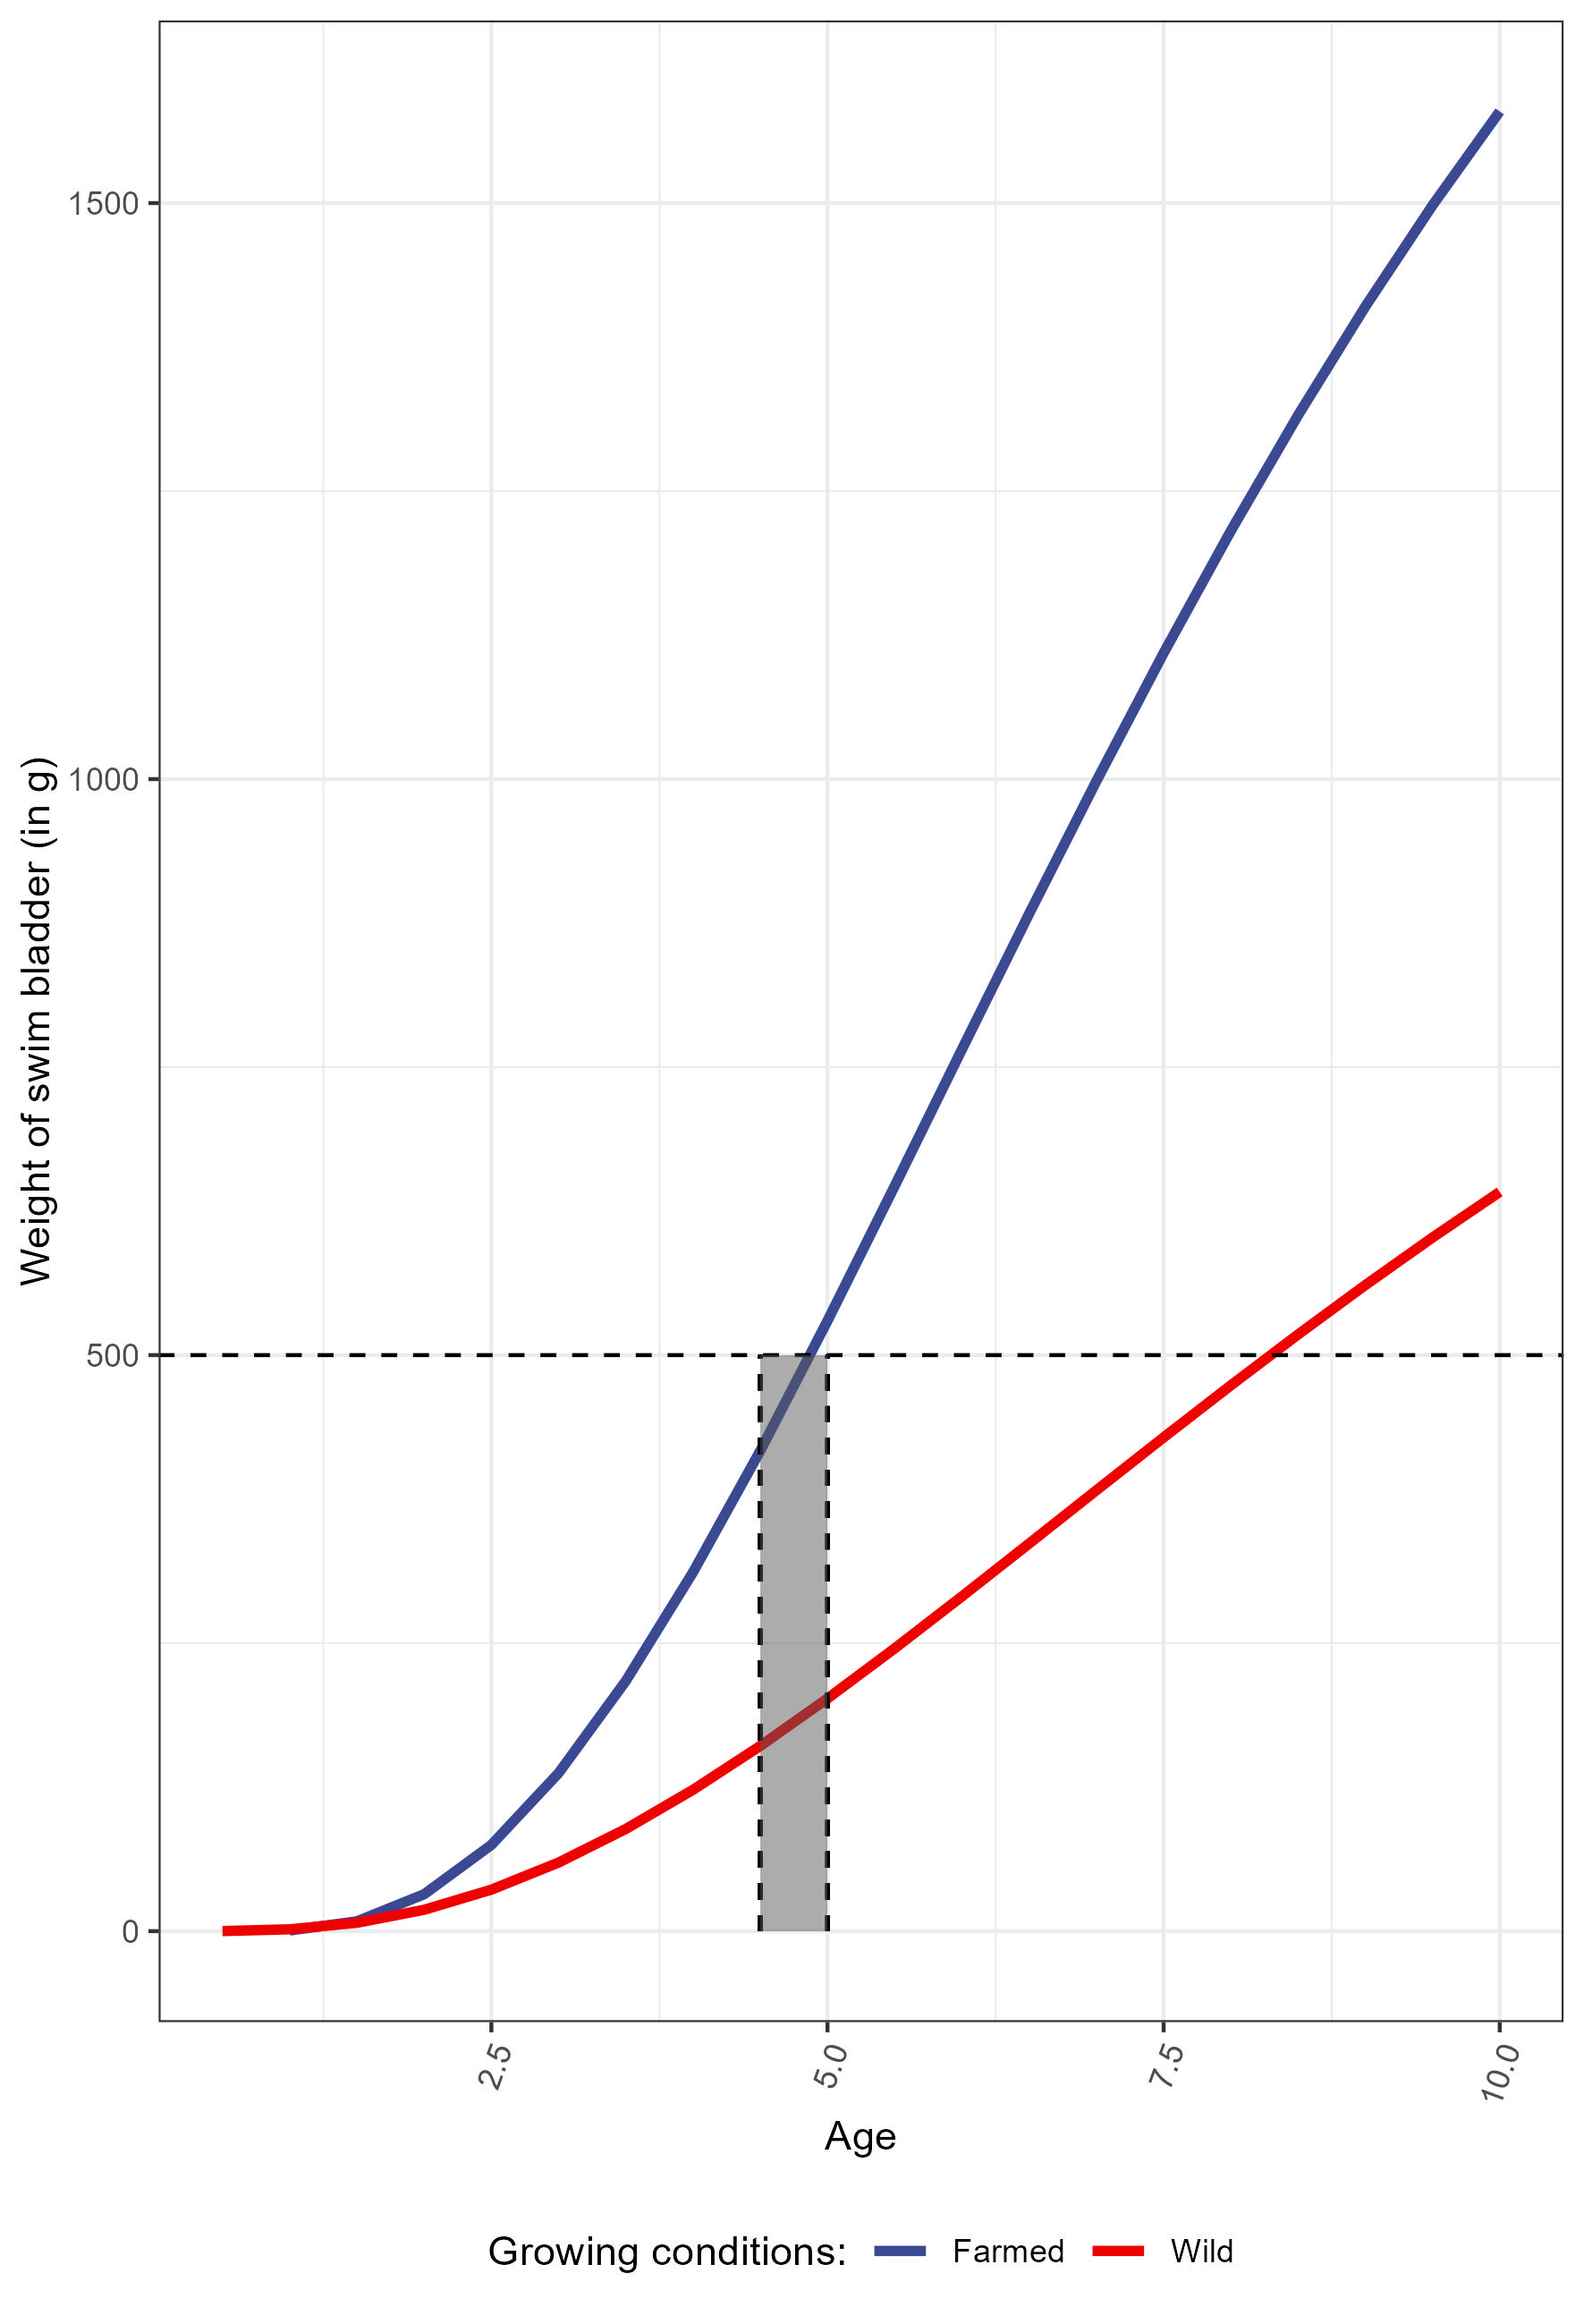
\includegraphics[width = .7\textwidth]{figures/totoaba/sup_fig4_VBGF_growth.jpg}
    \caption{Von Bertalanffy Growth curves for wild and farmed \textit{Totoaba macdonaldi} under different growing conditions}
    \subcaption*{
    Gray box indicates the range of ages that possess a 500 gram swim bladder. The wild individual growth curve was calibrated with information from the stock assessment, while the farmed individual growth curve was calibrated using}
    \label{fig:vbgf}
\end{figure}


\newpage

\begin{landscape}
\begin{table}[H]
%\caption{}
\centering
\begin{tabular}[t]{ccccc}
\hline 
Variable & Low Season & Mid Season & High Season & Source\\
\hline \hline
Vessels & 5 & 20 & 50 & \cite{cisneros-mata_evaluacion_2020} \\
Days per month & 4 & 12 & 14 & \cite{cisneros-mata_evaluacion_2020}\\
Total fleet days year & 20 & 240 & 700 & \cite{cisneros-mata_evaluacion_2020}\\
Food fuel day & 525 & 525 & 525 & Semi-Structured Interviews\\
Totoaba gearset & 2 & 3 & 6 & \cite{cisneros-mata_evaluacion_2020}\\
Gear loss day & 0.5 & 0.5 & 0.5 & Semi-Structured Interviews\\
Gearset vessel per day & 2 & 3 & 3 & \cite{cisneros-mata_evaluacion_2020}\\
Gear replacement & 1600 & 1600 & 1600 & Semi-Structured Interviews\\
Bribes/year & 600 & 7200 & 21000 & Semi-Structured Interviews\\
\hline 
Average cost (per vessel day) & 8385.34 & 14386.69 & 5051.26 & Authors' calculation\\
\hline \hline
\end{tabular}
\caption{Supporting information for the calculation of the\textit{ Totoaba macdonaldi} poaching cost parameters ($W_1$ and $W_2$)}
\subcaption*{The methods section details how and when semi-structured
 interviews were conducted.}
\label{tab:costW}
\end{table}
\end{landscape}
\newpage

\begin{landscape}
\begin{table}[H] 
\centering 
%  \caption{} 
\begin{tabular}{@{\extracolsep{5pt}}lc} 
\\[-1.8ex]\hline 
\hline \\[-1.8ex] 
 & \multicolumn{1}{c}{\textit{Dependent variable:}} \\ 
\cline{2-2} 
\\[-1.8ex] & Price \\ 
\hline \\[-1.8ex] 
 Catch & $-$1,563.752$^{**}$ \\ 
  & (725.985) \\ 
  & \\ 
 Constant & 1,625,837.000$^{***}$ \\ 
  & (406,789.500) \\ 
  & \\ 
\hline \\[-1.8ex] 
Observations & 45 \\ 
R$^{2}$ & 0.097 \\ 
Adjusted R$^{2}$ & 0.076 \\ 
Residual Std. Error & 431,737.700 (df = 43) \\ 
F Statistic & 4.640$^{**}$ (df = 1; 43) \\ 
\hline 
\hline \\[-1.8ex] 
\textit{Note:}  & \multicolumn{1}{r}{$^{*}$p$<$0.1; $^{**}$p$<$0.05; $^{***}$p$<$0.01} \\ 
\end{tabular} 
\caption{Regression output for the linear demand estimation calculated by regressing price data on catch data. }
\subcaption*{Data were obtained from the available literature that provided estimated weight and value
 of \textit{Totoaba macdonaldi} maw seizures on estimated \textit{Totoaba macdonaldi} catch from 2014 to 2017
 obtained from a recent stock assessment. The methods section details where information was obtained from. }
\label{tab:demand}
\end{table} 
\end{landscape}
\newpage

\begin{landscape}
\begin{table}[H]

\centering
\begin{tabular}[t]{ccc}
\hline
Variable & Value & Source\\
\hline\hline
Sphere & 1.00 & Earth Ocean Farm Video, 2022\\
Capacity per sphere (t) & 144.00 & Earth Ocean Farm Video, 2022\\
\hline \hline
\textit{In \$USD} & & \\
\hline
Maintenance year & 12500.00 & Felipe Ramirez, InnovaSea, 2018\\
Cleaning year & 5000.00 & Felipe Ramirez, InnovaSea, 2018\\
Vessel maintenance/year & 10000.00 & Tyler Korte, BlueOcean Mariculture, 2018;\\
& & 
Fernando Cavalin, Earth Ocean Farms, 2018\\
Fuel year & 25122.50 & Author's Calculations\\
Feed & 312480.00 & Tyler Korte, BlueOcean Mariculture, 2018\\
Labor & 1580000.00 & Authors' calculations\\
Facility lease & 150000.00 & Cygnus Ocean Farms, 2017\\
Admin. & 50000.00 & Cygnus Ocean Farms, 2017\\
\hline
Operational costs & 2145102.50 & Authors' calculations\\
Operational costs (per t \& year) & 14896.55 & Authors' calculations \\
\hline
\end{tabular}
\caption{Supporting information for the calculation of the \textit{Totoaba macdonaldi} farming cost parameter ($v$)}

\subcaption*{Annual cost estimates were obtained from informants and converted to \$USD. Capacity of each farming pen was obtained from Earth Ocean Farms, and an annual cost
706 per tonne of totoaba was calibrated using personal communications with totoaba aquaculture producers.}
\label{tab:costv}
\end{table}
\end{landscape}

\newpage



%\begin{table}[H]
%\centering
%\begin{tabular}[t]{cccc}
%\hline
%Parameter & Value & Concept & Units\\
%\hline \hline
%$\alpha$ & 1625836.98 & Demand model : intercept & USD\\

%$\beta$ & 1563.75 & Demand model : coefficient & USD/metric ton of biomass\\

%$r$ & 0.20 & Intrinsic growth rate & unitless\\

%$K$ & 20226.00 & Carrying capacity (in metric tons)   & \% of biomass/vessel trip\\

%$\sigma$ & $2\times 10^{-5}$ & Catchability & metric tons of biomass\\

%$Avg cost $& 8385.34 & Average cost per vessel trip & USD\\

%$W_{mid}$ & 2.18 & Parameter cost ($MC = Avg$) at historical value - middle & USD\\

%$W_{low}$ & 1.32 & Parameter cost ($MC = Avg$) at historical value - low & USD\\

%$W_{high}$ & 3.75 & Parameter cost ($MC = Avg$) at historical value - high & USD\\

%$Age$ & 4.50 & Age of farmed totoaba & Years\\

%$\gamma$ & 1407.38 & Substitutability & Unitless\\

%$v$ & 67034.45 & Unit cost of farming & USD/metric ton of biomass\\

%$c$ & 0.00 & Unit cost of trading & USD/ metric ton of biomass\\
%\hline
%\end{tabular}
%\caption{Summary of \textit{Totoaba macdonaldi} ecological and market parameters for model calibration}
%\subcaption*{The methods section details where information was obtained to estimate each parameter, as well as relevant equations.}
%\label{tab:params}


\begin{landscape}

\begin{table}[h]
\centering
\begin{tabular}[t]{c c c c}
\hline
Parameter & Value & Concept & Units\\
\hline \hline
$\alpha$ & 1,625,836.98 & Demand model : intercept & USD\\

$\beta$ & 1,563.75 & Demand model : coefficient & USD/metric ton of biomass\\

$\gamma$ & 1,354.25 & Demand model : substitutable good coefficient & USD/metric ton of biomass\\

\hline

$r$ & 0.20 & Intrinsic growth rate & unitless\\

$K$ & 20,226.00 & Carrying capacity (in metric tons) & metric tons of biomass\\

\hline 

$\sigma$ & $2\times 10^{-5}$ & Catchability & \% of biomass/vessel trip\\

$Avg Cost$ & 14,386.69 & Average cost per vessel trip at historical value & USD/vessel trip\\

$W$ & 3.75 & Quadratic cost parameter - Quadratic cost function & USD vessel trip$^{-2}$\\

$W_1$ & 12200.00 & Linear cost parameter - Linear quadratic cost function & USD/vessel trip\\

$W_2$ & 0.57 & Quadratic cost parameter - Linear quadratic cost function & USD vessel trip$^{-2}$\\

\hline 

$v$ & 89929.92 & Unit cost of farming & USD/metric ton of biomass\\

$i_r$ & 0.10 & Interest rate & \%\\

$Age$ & 4.50 & Age of farmed totoaba & Years\\
\hline 
$c$ & 0.00 & Unit cost of trading & USD/ metric ton of biomass\\
\hline \hline
\end{tabular}

\caption{Summary of \textit{Totoaba macdonaldi} ecological and market parameters for model calibration}
\subcaption*{The methods section details where information was obtained to estimate each parameter, as well as relevant equations.}
\label{tab:params}
\end{table}
\end{landscape}
\newpage

\begin{landscape}
    
\begin{table}[h]
    \centering
    \begin{tabular}{c c c}
    \hline \hline 
     Concept    & Formula  & Reference  \\
     \hline
     \textit{Fishery} &  & \\
     Growth & $ \dot{x} = rx\left(1 - \frac{x}{K}\right) - \sigma x E$ & eq. \ref{eq:growth}\\
     \hline
     \textit{Poaching}&  $s$ is price paid to poachers  & \\
     Harvest technology & $q = \sigma x E$ & \\
     Profit    & $\Pi = s \times (\sigma x E) - W_1 E - W_2 E^2$ &  \\
     Poached harvest & $q^W = \frac{s\sigma ^2 x - W_1}{2W_2}$ & eq. \ref{eq:poachers_supply}\\
     \\
     \hline 
     \textit{Vertical monopoly scenario}& \\
     Demand & $ P^m = \alpha^m - \beta^m q $ & eq. \ref{eq:inv_demand_monop} \\
     Profit & $\Pi^m = (P^m - s - c)q$ & eq. \ref{eq:profit_monop}\\
     Supply on end market & $q^*_m(x) =\frac{\sigma^2 x^2 (\alpha_m - c) - W_1 \sigma x}{2(\sigma^2 x^2 \beta^m +W_2)} $ & eq. \ref{eq:harvest_monop}
     \\
     \\
     \hline
     \textit{Duopoly} & &\\
     Aquaculture profit & $\Pi^F = (P^F - v)q^F$ & eq. \ref{eq:profit_aquaculture} \\
     Demand for imperfect substitutes & $P^W = \alpha^W- \beta^W q^W - \gamma q^F $ & eq. \ref{eq:demand_wild}\\
     
     & $P^F = \alpha^F
 - \beta^F q^F - \gamma q^W $ & eq. \ref{eq:demand_farmed}\\
    Quantity adjustment (Cournot) supply & $q^{W*}_C(x) = \frac{\sigma^2 x^2(2\beta^F(\alpha^W -c) - \gamma(\alpha^F - v)) - 2\beta^F W_1 \sigma x}{4 W_2 \beta^F + \sigma^2 x^2(4\beta^W \beta^F - \gamma^2)}$ & eq. \ref{eq:poaching_cournot}\\
    Price setting (Bertrand) supply & $q^{W*}_B(x) = \frac{b^W[\sigma^2 x^2 \big(b^F (2a^W + ev) + ea^F + c(e^2 - 2b^Wb^F)\big) - W_1 \sigma x (2b^F b^W - e^2)]}{2Wb^W (2b^Wb^F - e^2) + (4b^Fb^W - e^2) \sigma^2 x^2}$ & eq. \ref{eq:poaching_bertrand}\\
    \hline \hline  
    \end{tabular}
    \caption{Summary of the key functions in the model}
    \subcaption*{For model conclusions, the plotted functions are growth, vertical monopoly end market supply ($q^m$), quantity adjustment end market supply ($q^W_C$) and price setting end market supply ($q^W_B$)}
    \label{tab:totoaba_functions}
\end{table}
\end{landscape}

